\chapter{Experimentation}
\label{chap:experiments}
This chapter deals with the experiments, their design, execution and results.

 
\section{Experimental Design}
This section deals the specification of the Android benchmark app, used hardware, frameworks, models and how the measurements are conducted. 
Figure \ref{fig:expDesign} depicts a brief overview of the specifications of the experiments.
We use image classification as the use case, therefore an image needs to be sent to the model.
\begin{figure}[H]
\centering
\resizebox{.95\linewidth}{!}{

\tikzset{every picture/.style={line width=0.75pt}} %set default line width to 0.75pt        

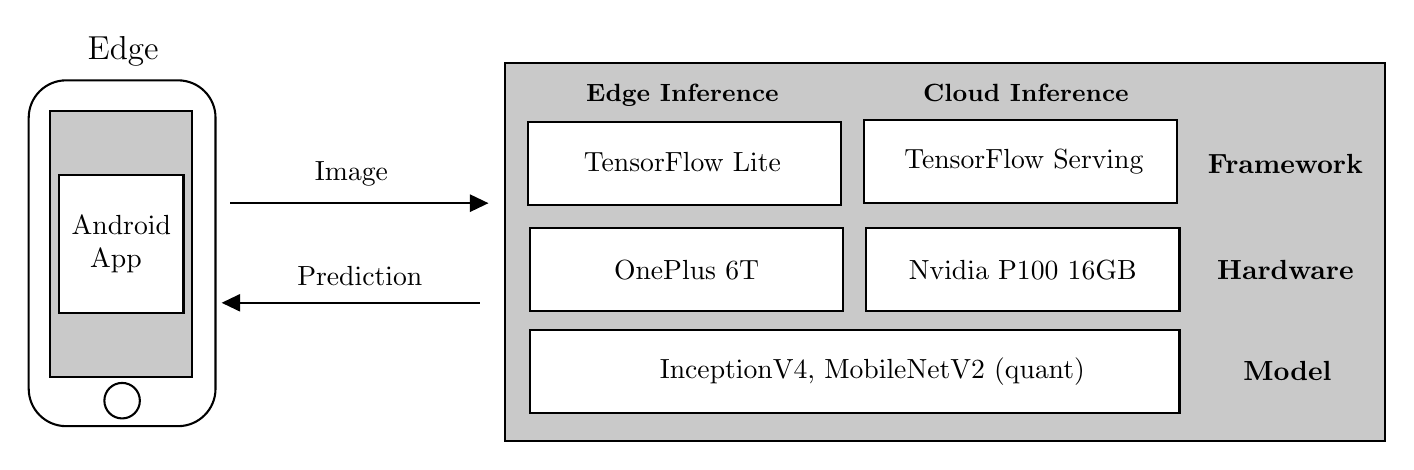
\begin{tikzpicture}[x=0.75pt,y=0.75pt,yscale=-1,xscale=1]
%uncomment if require: \path (0,485.57142639160156); %set diagram left start at 0, and has height of 485.57142639160156

%Straight Lines [id:da9993479608904674] 
\draw    (100.48,89) -- (223,89) ;
\draw [shift={(225,89)}, rotate = 540] [fill={rgb, 255:red, 0; green, 0; blue, 0 }  ][line width=0.75]  [draw opacity=0] (8.93,-4.29) -- (0,0) -- (8.93,4.29) -- cycle    ;

%Straight Lines [id:da5401559459790608] 
\draw    (98.48,137) -- (221,137) ;

\draw [shift={(96.48,137)}, rotate = 360] [fill={rgb, 255:red, 0; green, 0; blue, 0 }  ][line width=0.75]  [draw opacity=0] (8.93,-4.29) -- (0,0) -- (8.93,4.29) -- cycle    ;
%Shape: Rectangle [id:dp45054130026891115] 
\draw  [fill={rgb, 255:red, 201; green, 201; blue, 201 }  ,fill opacity=1 ] (233,21.57) -- (656.93,21.57) -- (656.93,203.57) -- (233,203.57) -- cycle ;
%Shape: Rectangle [id:dp21016153851852382] 
\draw  [fill={rgb, 255:red, 255; green, 255; blue, 255 }  ,fill opacity=1 ] (245,150) -- (557.93,150) -- (557.93,190) -- (245,190) -- cycle ;
%Shape: Rectangle [id:dp17739269402878732] 
\draw  [fill={rgb, 255:red, 255; green, 255; blue, 255 }  ,fill opacity=1 ] (244,50) -- (394.93,50) -- (394.93,90) -- (244,90) -- cycle ;
%Shape: Rectangle [id:dp9093436455970001] 
\draw  [fill={rgb, 255:red, 255; green, 255; blue, 255 }  ,fill opacity=1 ] (406,49) -- (556.93,49) -- (556.93,89) -- (406,89) -- cycle ;
%Shape: Rectangle [id:dp14120602080303146] 
\draw  [fill={rgb, 255:red, 255; green, 255; blue, 255 }  ,fill opacity=1 ] (245,101) -- (395.93,101) -- (395.93,141) -- (245,141) -- cycle ;
%Shape: Rectangle [id:dp45473714544487454] 
\draw  [fill={rgb, 255:red, 255; green, 255; blue, 255 }  ,fill opacity=1 ] (407,101) -- (557.93,101) -- (557.93,141) -- (407,141) -- cycle ;
%Shape: Rectangle [id:dp4153343207585154] 
\draw  [fill={rgb, 255:red, 201; green, 201; blue, 201 }  ,fill opacity=1 ] (13.91,44.69) -- (82.34,44.69) -- (82.34,172.63) -- (13.91,172.63) -- cycle ;
%Rounded Rect [id:dp09380596237315397] 
\draw   (3.5,47.82) .. controls (3.5,37.88) and (11.56,29.82) .. (21.5,29.82) -- (75.5,29.82) .. controls (85.44,29.82) and (93.5,37.88) .. (93.5,47.82) -- (93.5,178.43) .. controls (93.5,188.37) and (85.44,196.43) .. (75.5,196.43) -- (21.5,196.43) .. controls (11.56,196.43) and (3.5,188.37) .. (3.5,178.43) -- cycle ;
%Shape: Ellipse [id:dp8964060056788943] 
\draw   (39.95,184.16) .. controls (39.95,179.43) and (43.78,175.6) .. (48.5,175.6) .. controls (53.22,175.6) and (57.05,179.43) .. (57.05,184.16) .. controls (57.05,188.88) and (53.22,192.71) .. (48.5,192.71) .. controls (43.78,192.71) and (39.95,188.88) .. (39.95,184.16) -- cycle ;
%Shape: Rectangle [id:dp85708751067272] 
\draw  [fill={rgb, 255:red, 255; green, 255; blue, 255 }  ,fill opacity=1 ] (18.19,75.22) -- (78.07,75.22) -- (78.07,142.1) -- (18.19,142.1) -- cycle ;

% Text Node
\draw (159,75) node  [align=left] {Image};
% Text Node
\draw (163,124) node  [align=left] {Prediction};
% Text Node
\draw (49,16) node  [align=left] {{\large Edge}};
% Text Node
\draw (409.96,170) node  [align=left] {InceptionV4, MobileNetV2 (quant)};
% Text Node
\draw (318.46,37) node  [align=left] {{\small \textbf{Edge Inference}}};
% Text Node
\draw (483.96,36) node  [align=left] {{\small \textbf{Cloud Inference}}};
% Text Node
\draw (318.46,69) node  [align=left] {TensorFlow Lite};
% Text Node
\draw (482.96,68.79) node  [align=left] {TensorFlow Serving};
% Text Node
\draw (320.46,121) node  [align=left] {OnePlus 6T};
% Text Node
\draw (482.46,121) node  [align=left] {Nvidia P100 16GB};
% Text Node
\draw (608.96,70) node  [align=left] {\textbf{Framework}};
% Text Node
\draw (608.96,121) node  [align=left] {\textbf{Hardware}};
% Text Node
\draw (609.96,170) node  [align=left] {\textbf{Model}};
% Text Node
\draw (48.13,108.66) node  [align=left] {Android\\ \ \ App};


\end{tikzpicture}}
\caption{Experimental Design}
\label{fig:expDesign}
\end{figure}


\subsection{Hardware Devices}
\subsubsection{Edge}
\label{chap:hardwareEdge}
As the edge device we will use the OnePlus 6T (ONEPLUS A6013). This state of the art smartphone is powered by a Qualcomm Snapdragon 845 CPU(Octa-core, up to 2.8 GHz), Adreno 630 GPU, 8 GB of memory and runs on OxygenOS 9.0.11, which is based on Android 9.
%%Cite from AI bechmark paper
\subsubsection{Cloud}
%The Nvidia DGX-1 will serve as the cloud-backend for the experiments. This server consists of 8$\times$Tesla V100 providing 1000 TFLOPS as well as 256 GB GPU memory and 512 GB system memory.
The virtual server has 32 cores (16 real cores with hyperthreading), 240 GB of memory, a Tesla P100 16 GB PCIe GPGPU and a 800 PCIe SSD.

The server runs on Ubuntu 16.04 CUDA 9.1 PGI 17.9 nvidia-docker 2.0.3+docker18.03.1-1.
\subsection{Deep Learning Inference Framework}
We use two open source machine learning frameworks based on TensorFlow for the experiments, TensorFlow Lite and TensorFlow Serving. We decided to use these framework because they are open source and support, at the point of this theses, the operations for most image classification models and also a increasing number of hardware accelerators and operating systems for both edge and cloud inference.
TensorFlow provides official releases, that are maintained and tested, of the models we like to evaluate
This section only gives a brief overview of the most important aspects of the frameworks, for detailed information consider the TensorFlow Lite\cite{tfLite}  and TensorFlow Serving\cite{tfServing} websites, on which this section is based on, or the corresponding GitHub repositories
We chose these frameworks since they both support TensorFlow models, ...%INSERT more reason here
\subsubsection{TensorFlow Lite}
\label{chap:TFLite}
TensorFlow Lite (Release 1.12.0) was developed for mobile and embedded devices and is a lightweight solution of TensorFlow and thus will be used for the edge inference experiments.

%%Mention NNAPI support?
At the moment only model inference can be done by TensorFlow Lite, not model training.
It supports acceleration with GPU or other accelerators as well was portability to Android, iOS and other IoT devices.

\paragraph{Android NNAPI}
\label{chap:NNAPI}
TensorFlow Lite is also compatible with the Android Neural Networks API (NNAPI). This API
is designed to speed up computationally intensive machine learning operations and can be used by TensorFlow Lite to improve inference performance. During inference NNAPI "can
efficiently distribute the computation workload across available on-device processors, including dedicated neural network chips, GPUs and DSPs"\cite{DBLP:journals/corr/abs-1810-01109}.



\paragraph{Hosting Models}
TensorFlow Lite expects models in their own FlatBuffer file  format(\emph{.tflite}). Therefore models need to be converted to this format before TensorFlow Lite can load them. This conversion can be done using the TensorFlow Lite Converter, which supports various formats of trained TensorFlow models.
The \emph{.tflite} model now can be loaded by a object of the Interpreter class.
\paragraph{Run Prediction}

To then run the inference process in TensorFlow Lite the run method of Interpreter object with a loaded model needs to be called. To call this function two objects need to be passed, first the input for the given model and second the output object, where the prediction response from the inference operation gets stored. 
\begin{figure}[H]
\centering



\tikzset{every picture/.style={line width=0.75pt}} %set default line width to 0.75pt        

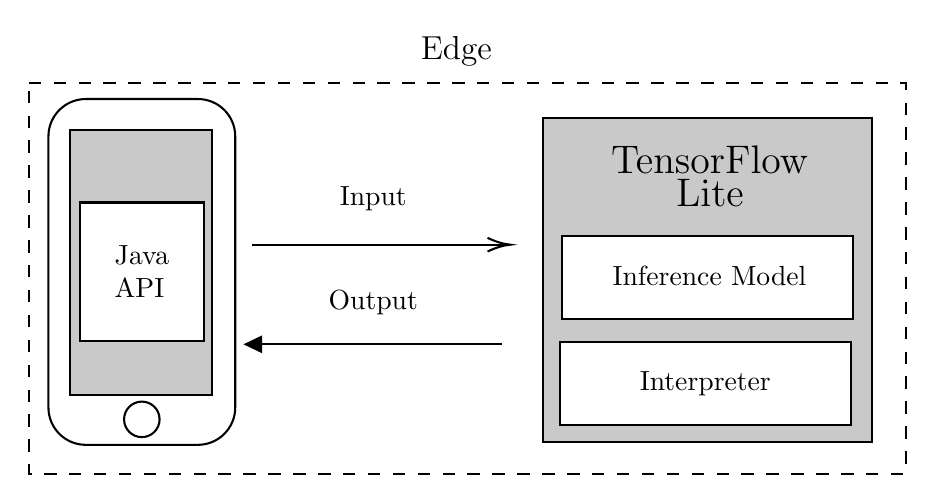
\begin{tikzpicture}[x=0.75pt,y=0.75pt,yscale=-1,xscale=1]
%uncomment if require: \path (0,300); %set diagram left start at 0, and has height of 300

%Shape: Rectangle [id:dp13292222689234756] 
\draw  [fill={rgb, 255:red, 201; green, 201; blue, 201 }  ,fill opacity=1 ] (61.91,111.69) -- (130.34,111.69) -- (130.34,239.63) -- (61.91,239.63) -- cycle ;
%Rounded Rect [id:dp7897713915001106] 
\draw   (51.5,114.82) .. controls (51.5,104.88) and (59.56,96.82) .. (69.5,96.82) -- (123.5,96.82) .. controls (133.44,96.82) and (141.5,104.88) .. (141.5,114.82) -- (141.5,245.43) .. controls (141.5,255.37) and (133.44,263.43) .. (123.5,263.43) -- (69.5,263.43) .. controls (59.56,263.43) and (51.5,255.37) .. (51.5,245.43) -- cycle ;
%Shape: Ellipse [id:dp9670901006981827] 
\draw   (87.95,251.16) .. controls (87.95,246.43) and (91.78,242.6) .. (96.5,242.6) .. controls (101.22,242.6) and (105.05,246.43) .. (105.05,251.16) .. controls (105.05,255.88) and (101.22,259.71) .. (96.5,259.71) .. controls (91.78,259.71) and (87.95,255.88) .. (87.95,251.16) -- cycle ;
%Straight Lines [id:da9993479608904674] 
\draw    (149.48,167) -- (272,167) ;
\draw [shift={(274,167)}, rotate = 540] [color={rgb, 255:red, 0; green, 0; blue, 0 }  ][line width=0.75]    (10.93,-3.29) .. controls (6.95,-1.4) and (3.31,-0.3) .. (0,0) .. controls (3.31,0.3) and (6.95,1.4) .. (10.93,3.29)   ;

%Straight Lines [id:da5401559459790608] 
\draw    (147.48,215) -- (270,215) ;

\draw [shift={(145.48,215)}, rotate = 360] [fill={rgb, 255:red, 0; green, 0; blue, 0 }  ][line width=0.75]  [draw opacity=0] (8.93,-4.29) -- (0,0) -- (8.93,4.29) -- cycle    ;
%Shape: Rectangle [id:dp45054130026891115] 
\draw  [fill={rgb, 255:red, 201; green, 201; blue, 201 }  ,fill opacity=1 ] (290,106) -- (448.5,106) -- (448.5,262) -- (290,262) -- cycle ;
%Shape: Rectangle [id:dp21016153851852382] 
\draw  [fill={rgb, 255:red, 255; green, 255; blue, 255 }  ,fill opacity=1 ] (299,163) -- (439,163) -- (439,203) -- (299,203) -- cycle ;
%Shape: Rectangle [id:dp8946256165796296] 
\draw  [fill={rgb, 255:red, 255; green, 255; blue, 255 }  ,fill opacity=1 ] (298,214) -- (438,214) -- (438,254) -- (298,254) -- cycle ;
%Shape: Rectangle [id:dp1345031923489386] 
\draw  [dash pattern={on 4.5pt off 4.5pt}] (42,89) -- (464.5,89) -- (464.5,277.4) -- (42,277.4) -- cycle ;
%Shape: Rectangle [id:dp7242946292477495] 
\draw  [fill={rgb, 255:red, 255; green, 255; blue, 255 }  ,fill opacity=1 ] (66.56,146.69) -- (126.44,146.69) -- (126.44,213.56) -- (66.56,213.56) -- cycle ;

% Text Node
\draw (208,145) node  [align=left] {Input};
% Text Node
\draw (248,74) node  [align=left] {{\large Edge}};
% Text Node
\draw (370,134) node  [align=left] {{\Large TensorFlow}\\{\Large  \ \ \ \ \ Lite}};
% Text Node
\draw (370,182) node  [align=left] {Inference Model};
% Text Node
\draw (208,195) node  [align=left] {Output};
% Text Node
\draw (368,234) node  [align=left] {Interpreter};
% Text Node
\draw (96.5,180.12) node  [align=left] {Java\\ API};


\end{tikzpicture}
\caption{Functionality of TensorFlow Lite}
\label{fig:edge}
\end{figure}
\subsubsection{TensorFlow Serving}
\label{chap:TFServing}
As for cloud inference TensorFlow Serving (Release 1.12.0 VERIFY THIS AGAIN) will be used, since it provides a framework to serve machine learning models in production environments. 



\paragraph{Hosting Models}
In order to host a model as a Servable in TensorFlow Serving, first a TensorFlow model needs to exported using TensorFlow's SavedModelBuilder, resulting in a SavedModel protocol buffer file along with the model’s variables and assets (Although TensorFlow Serving is optimized for TensorFlow models, the framework can be extended to serve other types of models).
%%Wieviel schreiben über signature, predict function etc?

Now the exported model can be loaded by a instance of Tensorflow Serving.
We use docker to start that instance, specifically nvidia-docker that allows us to run the inference operations on a GPU. For that TensorFlow Serving provides two docker images of their framework, one with CPU and the other with GPU support.

\paragraph{Run Prediction}
TensorFlow Serving supports two API for clients to create predictions requests: gRPC and REST. Since the gRPC protocol is supposed to deliver a better performance, we will use the gRPC API.
For a client to a request to the server a gRPC stub needs to be created in the first place, that allows us to call all methods implemented on the server. In our case we need to call TensorFlow Serving's Predict method to start the inference process. The method needs to be passed a PredictRequest object, which contains among other things the input data for the model, the shape of the input and the requested model.%model signature?

After the request is sent and handled the server response by sending back a PredictResponse object. This object holds the predictions for the given input data in the form specified by the exported model.
This request and response process can also be seen in figure \ref{fig:cloud}

\begin{figure}[H]
\centering


\tikzset{every picture/.style={line width=0.75pt}} %set default line width to 0.75pt        

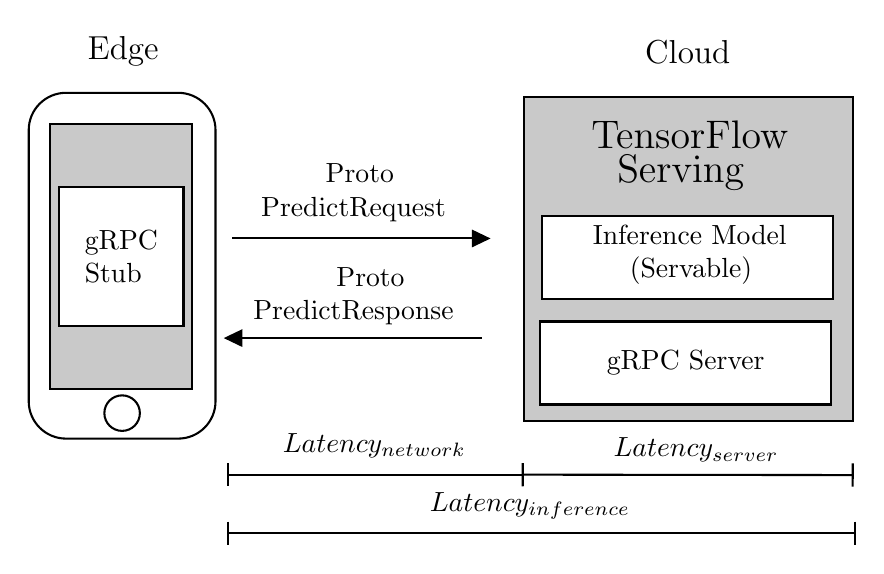
\begin{tikzpicture}[x=0.75pt,y=0.75pt,yscale=-1,xscale=1]
%uncomment if require: \path (0,300); %set diagram left start at 0, and has height of 300

%Straight Lines [id:da7072764839644827] 
\draw    (149.5,291) -- (451.5,291) ;
\draw [shift={(451.5,291)}, rotate = 180] [color={rgb, 255:red, 0; green, 0; blue, 0 }  ][line width=0.75]    (0,5.59) -- (0,-5.59)   ;
\draw [shift={(149.5,291)}, rotate = 180] [color={rgb, 255:red, 0; green, 0; blue, 0 }  ][line width=0.75]    (0,5.59) -- (0,-5.59)   ;
%Straight Lines [id:da9536138531960994] 
\draw    (291.5,262.8) -- (450.5,263) ;
\draw [shift={(450.5,263)}, rotate = 180.07] [color={rgb, 255:red, 0; green, 0; blue, 0 }  ][line width=0.75]    (0,5.59) -- (0,-5.59)   ;
\draw [shift={(291.5,262.8)}, rotate = 180.07] [color={rgb, 255:red, 0; green, 0; blue, 0 }  ][line width=0.75]    (0,5.59) -- (0,-5.59)   ;
%Shape: Rectangle [id:dp8902536871651789] 
\draw  [fill={rgb, 255:red, 201; green, 201; blue, 201 }  ,fill opacity=1 ] (63.91,93.69) -- (132.34,93.69) -- (132.34,221.63) -- (63.91,221.63) -- cycle ;
%Rounded Rect [id:dp41557214204551274] 
\draw   (53.5,96.82) .. controls (53.5,86.88) and (61.56,78.82) .. (71.5,78.82) -- (125.5,78.82) .. controls (135.44,78.82) and (143.5,86.88) .. (143.5,96.82) -- (143.5,227.43) .. controls (143.5,237.37) and (135.44,245.43) .. (125.5,245.43) -- (71.5,245.43) .. controls (61.56,245.43) and (53.5,237.37) .. (53.5,227.43) -- cycle ;
%Shape: Ellipse [id:dp8878397246816687] 
\draw   (89.95,233.16) .. controls (89.95,228.43) and (93.78,224.6) .. (98.5,224.6) .. controls (103.22,224.6) and (107.05,228.43) .. (107.05,233.16) .. controls (107.05,237.88) and (103.22,241.71) .. (98.5,241.71) .. controls (93.78,241.71) and (89.95,237.88) .. (89.95,233.16) -- cycle ;
%Straight Lines [id:da5813802620369573] 
\draw    (151.48,149) -- (274,149) ;
\draw [shift={(276,149)}, rotate = 540] [fill={rgb, 255:red, 0; green, 0; blue, 0 }  ][line width=0.75]  [draw opacity=0] (8.93,-4.29) -- (0,0) -- (8.93,4.29) -- cycle    ;

%Straight Lines [id:da16220168680973557] 
\draw    (149.48,197) -- (272,197) ;

\draw [shift={(147.48,197)}, rotate = 360] [fill={rgb, 255:red, 0; green, 0; blue, 0 }  ][line width=0.75]  [draw opacity=0] (8.93,-4.29) -- (0,0) -- (8.93,4.29) -- cycle    ;
%Shape: Rectangle [id:dp8411150472244695] 
\draw  [fill={rgb, 255:red, 201; green, 201; blue, 201 }  ,fill opacity=1 ] (292,81) -- (450.5,81) -- (450.5,237) -- (292,237) -- cycle ;
%Shape: Rectangle [id:dp13557861576626729] 
\draw  [fill={rgb, 255:red, 255; green, 255; blue, 255 }  ,fill opacity=1 ] (301,138) -- (441,138) -- (441,178) -- (301,178) -- cycle ;
%Shape: Rectangle [id:dp5681963435258506] 
\draw  [fill={rgb, 255:red, 255; green, 255; blue, 255 }  ,fill opacity=1 ] (68.19,124.22) -- (128.07,124.22) -- (128.07,191.1) -- (68.19,191.1) -- cycle ;
%Shape: Rectangle [id:dp7458124222136935] 
\draw  [fill={rgb, 255:red, 255; green, 255; blue, 255 }  ,fill opacity=1 ] (300,189) -- (440,189) -- (440,229) -- (300,229) -- cycle ;
%Straight Lines [id:da6846625455377753] 
\draw    (149.5,262.8) -- (291.5,262.8) ;
\draw [shift={(291.5,262.8)}, rotate = 180] [color={rgb, 255:red, 0; green, 0; blue, 0 }  ][line width=0.75]    (0,5.59) -- (0,-5.59)   ;
\draw [shift={(149.5,262.8)}, rotate = 180] [color={rgb, 255:red, 0; green, 0; blue, 0 }  ][line width=0.75]    (0,5.59) -- (0,-5.59)   ;

% Text Node
\draw (375,251) node  [align=left] {$\displaystyle Latency_{server}$$ $};
% Text Node
\draw (210,127) node  [align=left] { \ \ \ \ \ \ \ Proto\\PredictRequest};
% Text Node
\draw (99,59) node  [align=left] {{\large Edge}};
% Text Node
\draw (371,59) node  [align=left] {{\large Cloud}};
% Text Node
\draw (372,109) node  [align=left] {{\Large TensorFlow}\\{\Large  \ \ Serving}};
% Text Node
\draw (372,157) node  [align=left] {Inference Model\\ \ \ \ \ (Servable)};
% Text Node
\draw (210,177) node  [align=left] { \ \ \ \ \ \ \ \ \ Proto\\PredictResponse};
% Text Node
\draw (98.13,157.66) node  [align=left] {gRPC\\ Stub};
% Text Node
\draw (370,209) node  [align=left] {gRPC Server};
% Text Node
\draw (220,249) node  [align=left] {$\displaystyle Latency_{network}$$ $};
% Text Node
\draw (295,278) node  [align=left] {$\displaystyle Latency_{inference}$$ $};


\end{tikzpicture}
\caption{Functionality of TensorFlow Serving}
\label{fig:cloud}
\end{figure}
\subsection{Models}
\label{chap:models}
We will use two different image classification model for the experiment, one optimised for mobile deployment and the other towards high accuracy.
Both models are trained on a ImageNet dataset consisting of 1001 image classes.

For the TensorFlow Lite version we use the models provided on the TensorFlow Lite website \cite{tfLiteModels}.
To convert model suitable for TensorFlow Serving we use the TensorFlow-Slim library \cite{tfSlim}, where maintained and tested implementations of popular image classification models are being published. For both Serving and Lite we use the same training checkpoint to get the same weights for the graphs.


\subsubsection{MobileNetV2}
MobileNetV2 (version 1.0) is a successor of MobileNetV1 and is "specifically tailored for mobile and resource
constrained environments" \cite{DBLP:journals/corr/abs-1801-04381}. The authors do this by "significantly decreasing the number of operations and the memory needed while retaining the same accuracy"  \cite{DBLP:journals/corr/abs-1801-04381} and introducing a new layer module called "the
inverted residual with linear bottleneck" \cite{DBLP:journals/corr/abs-1801-04381}.
This module is a combination of 

Table \ref{table:mobilenetArchi} displays the design of the model, with each row being a layer repeated \emph{n} times. 
\begin{table}[]

\centering
\caption{MobilenetV2 architecture \cite{DBLP:journals/corr/abs-1801-04381}}
\label{table:mobilenetArchi}
\begin{tabular}{@{}llllll@{}}

\toprule
Input & Operator & t & c & n & s \\ \midrule
$224^2\times 3$ & conv2d & - & 32 & 1 & 2 \\
$112^2\times 32$ & bottleneck & 1 & 16 & 1 & 1 \\
$112^2\times 16$ & bottleneck & 6 & 24 & 2 & 2 \\
$56^2\times 24$ & bottleneck & 6 & 32 & 3 & 2 \\
$28^2\times 23$ & bottleneck & 6 & 64 & 4 & 2 \\
$14^2\times 64$ & bottleneck & 6 & 96 & 3 & 1 \\
$14^2\times 96$ & bottleneck & 6 & 160 & 3 & 2 \\
$7^2\times 160$ & bottleneck & 6 & 320 & 1 & 1 \\
$7^2\times 320$ & conv2d 1x1 & - & 1280 & 1 & 1 \\
$7^2\times 1280$ & avgpool 7x7 & - & - & 1 & - \\
$1\times 1\times 1280$ & conv2d 1x1 & - & k & - &  \\ \bottomrule
\end{tabular}
\end{table}
\paragraph{Quantization}
Quantization of MobileNetV2, using the techniques presented in section \ref{chap:quant}, results in a  0.7\% loss of top-5 accuracy, but therefore has lost 75\% of its model size and a optimised performance, which we will evaluate in the experiments.
\subsubsection{Inception V4}
%%Add infos about stem and reduction
InceptionV4, published in \cite{InceptionV4}, is a large image classification network with high accuracy but also with a high number of parameters leading to higher inference times than MobileNetV2.

In comparison to its previous versions InceptionV4 is built with "a more uniform simplified architecture and more inception modules". These inception modules consists of multiple convolutional, average pooling and filter concat layers.
The general architecture of the network can be seen in figure \ref{fig:inceptionv4} with different Inception and Reduction building blocks. 
\begin{figure}[]
\centering
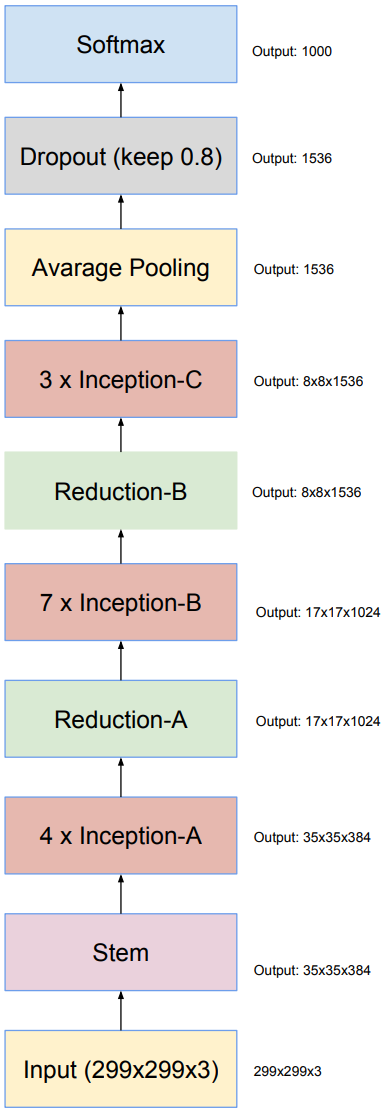
\includegraphics[angle=90,width=0.94\textwidth]{./Bilder/inceptionV4_architecture.png}
\caption{InceptionV4 architecture \cite{InceptionV4}}
\label{fig:inceptionv4}
\end{figure}
\begin{table}[]
%CITE inception params ned vergessen
\caption{Overview of used models}
\label{table:modelOverview}
\begin{tabular}{@{}lllll@{}}
\toprule
Model & Parameters & Top-5 Accuracy\cite{modelspecs} & Input Size & TF Lite Model Size \\
\midrule
InceptionV4 & 42.68M & 95.1\% & 299x299 & 107.7MB \\
MobileNetV2 1.0 & 3.47M\cite{DBLP:journals/corr/abs-1801-04381} & 90.6 & 224x224 & 14MB \\
MobileNetV2 1.0 & 3.47M\cite{DBLP:journals/corr/abs-1801-04381} & 89.9\% & 224x224 & 3.4MB\\
\bottomrule
\end{tabular}
\end{table}


\subsection{Android Benchmark Application}
To conduct the experiments for both edge and cloud inference we developed and implemented an Android benchmark application using Kotlin.
This application implements all function needed to preprocess real workload images and perform the inference on either the Android device itself or sent the image to a cloud-backend.
For both the preprocess and inference operation the application logs metrics such as inference latency, time of the experiments etc. and stores them to a \emph{CSV} file, which then can be used to analyze the experiments.

Both edge and cloud inference implementations are based on the example implementations in the respective GitHub repositories to ensure optimal performance. 

\begin{figure}[htb]
\centering
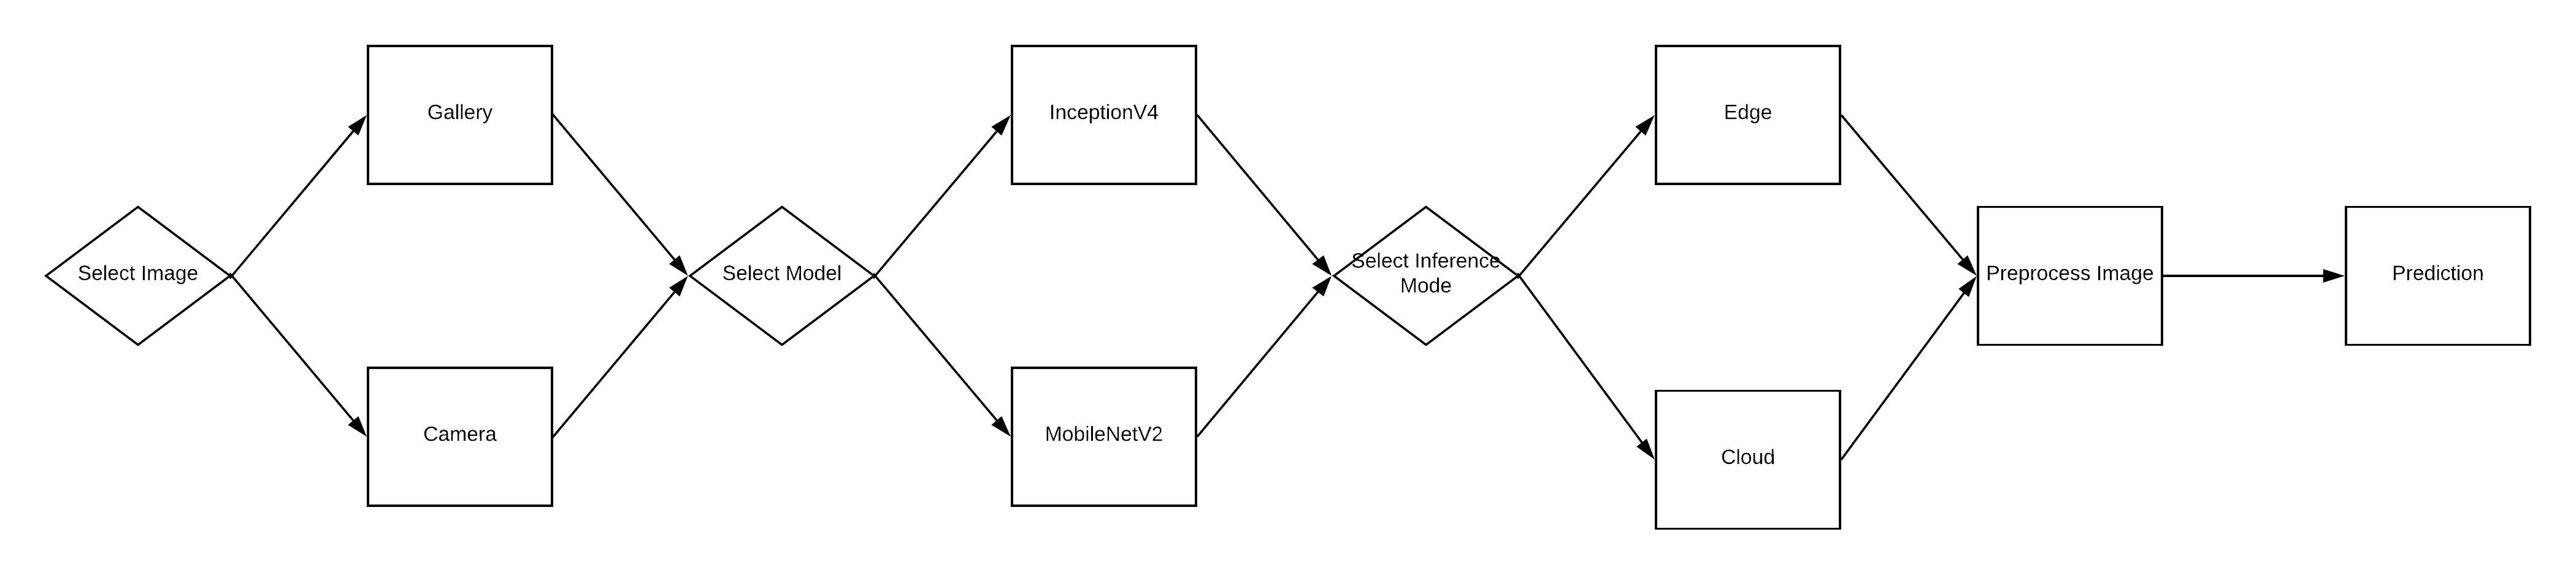
\includegraphics[width=0.95\textwidth]{./Bilder/FlowChart_App.png}
\caption{Flowchart of the Benchmark Application}
\label{fig:app}
\end{figure}
In figure \ref{fig:app} the workflow to perform the inference is seen. First, a image needs to be selected. Afterwards the image classification model needs to be chosen. Now the user selects whether the inference should be performed on the cloud-backend or directly on the edge device, in this case a android phone. In the case of edge inference it needs to be decided if the NNAPI should be used by TensorFlow Lite. For cloud inference the preprocessing mode needs to be selected (edge/cloud). Now the preprocessing operations can be performed based on the previous selected options (Even for the case of cloud inference with cloud preprocessing some preprocessing needs to be done on the edge beforehand like building the \emph{Proto PredictRequest}). Now, that the input is preprocessed, the actual inference is performed resulting in a prediction. For both preprocessing and inference the measurements mentioned in section \ref{chap:insta_measurements} are logged.

\begin{figure}[htb]
\centering
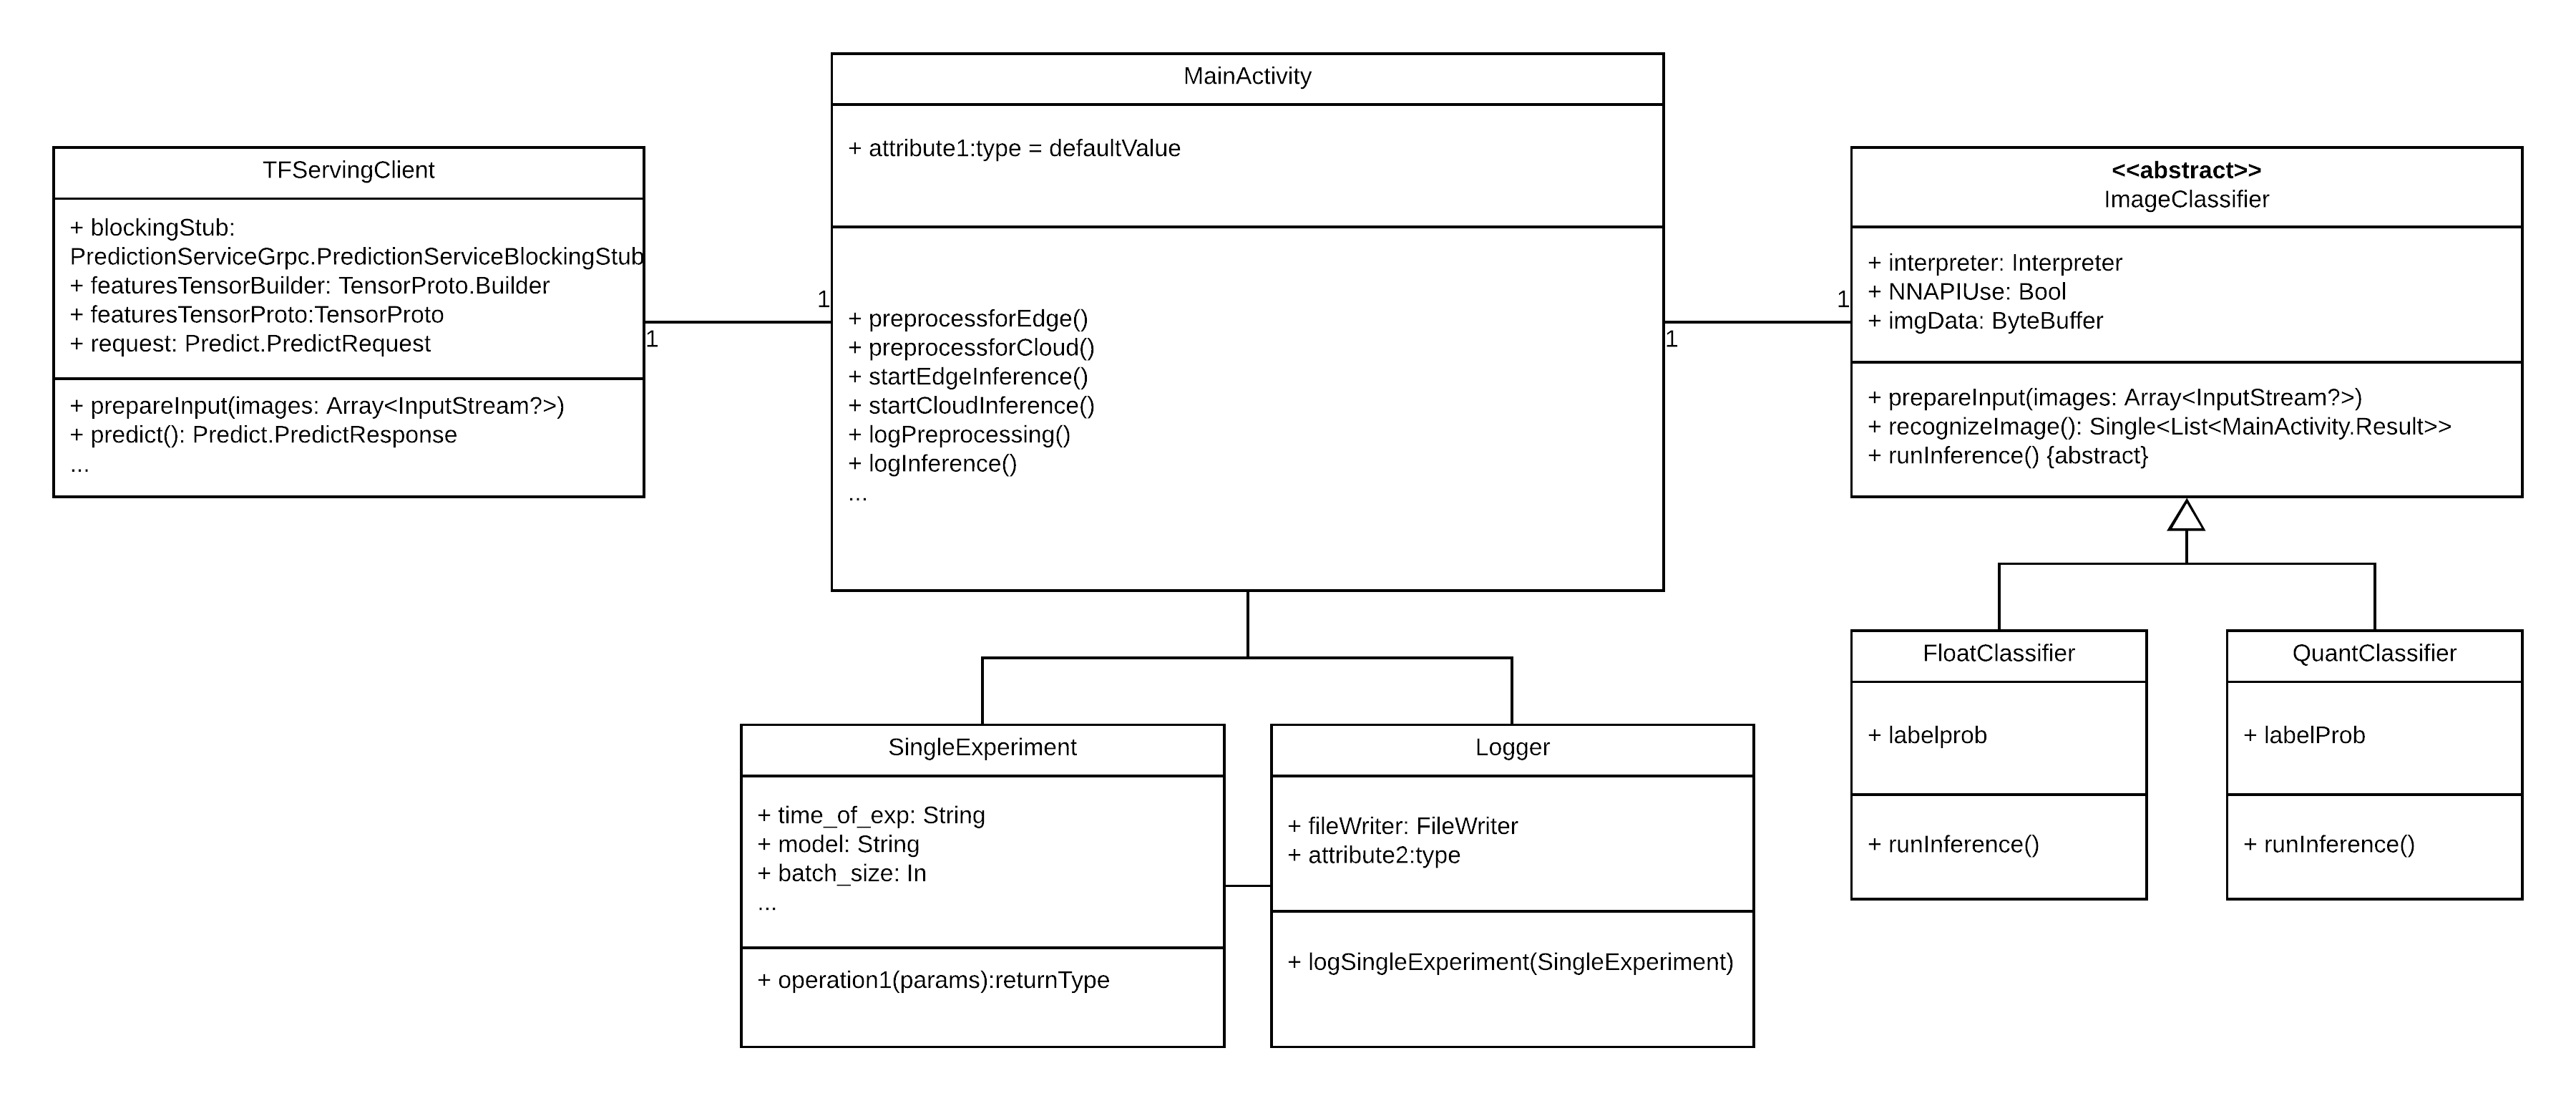
\includegraphics[width=0.95\textwidth]{./Bilder/UML.png}
\caption{UML class diagram of the benchmark Application}
\label{fig:UML}
\end{figure}
Figure \ref{fig:UML} depicts an UML class diagram of the application featuring the most important classes, functions and variables. 
The main class is called \emph{MainActivity} and implements all of the graphical aspects. 
The \emph{MainActivity} handles requests for both cloud and edge inference by delegating the requests to instances of the classes \emph{TFServingClient} and \emph{ImageClassifier}, respectively. Both of these classes also take care of the preprocessing steps.
The abstract class \emph{ImageClassifier} has two subclasses \emph{FloatClassifier} and \emph{QuantClassifier}. The first class runs the inference for floating point models and the second for quantized models.
This seperation is needed since these different model types require different input and output types.

The \emph{MainActivity} writes the collected measurements and the parameter configurations of a experiment to a instance of \emph{SingleExperiment}. After the experiment is completed \emph{MainActivity} tells a Logger instance to save the contents of the \emph{SingleExperiment} object. The Logger then saves all collected data to a \emph{CSV} file.

\subsubsection{Preprocessing}
%%mention png
For the case of image classification, the images need to have the correct size ($224\times224$ for MobilenetV2 and $299\times299$ for InceptionV4) and the RGB values need to be scaled to the interval $[-1,1]$. After preprocessing the image has been transformed into the shape $224\times224\times3$ with all values between $[-1,1]$, where the the first two dimensions represent the image height and width, while the last dimension represent the number of channels (3 since the images are rgb)
\begin{figure}[H]
\centering
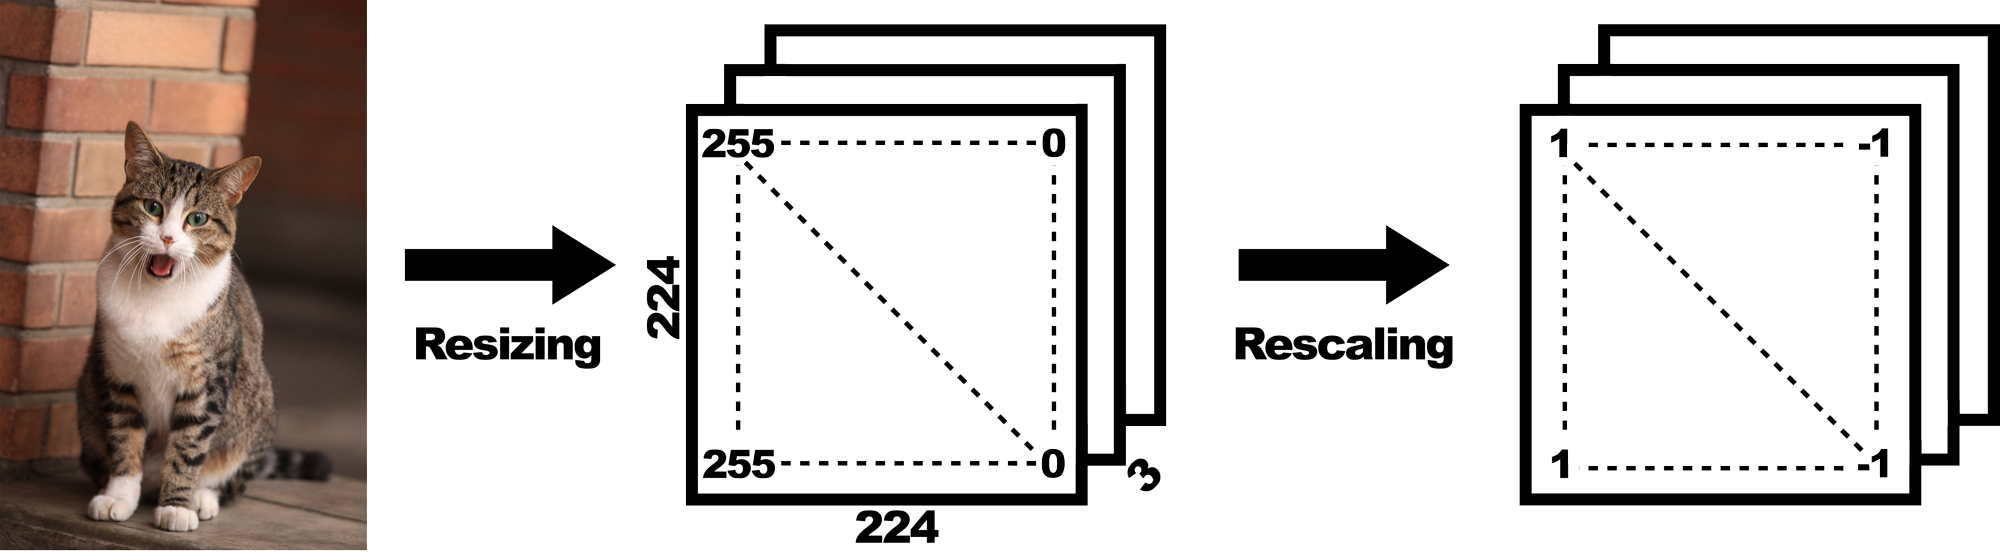
\includegraphics[width=0.8\textwidth]{./Bilder/preprocessing.png}
\caption{Preprocessing steps for image classifcation}
\label{fig:prepro}
\end{figure}
\paragraph{Edge Preprocessing}
In the case of edge preprocessing all preprocessing steps are done on the edge device, meaning that the input can be fed directly into the neural afterwards, either on the edge device itself or on a cloud-backend.
We perform these steps the following way: After loading the PNG image into an \emph{InputStream} we created a scaled Bitmap of the image (scaled to either $224\times224$ or $299\times299$). 
Afterwards we rescale the RGB values during the conversion from the bitmap to a \emph{ByteBuffer}. 
For the case of float models these buffer contain all the pixels in float format and for quantized model in bytes.
%%%mehr erklären?
We do this conversion since feeding \emph{ByteBuffers} to TensorFlow Lite is performance enhancing %add cite here
For cloud inference we then construct \emph{PredictRequest} object containing this \emph{ByteBuffer}.

For batch size larger than one we parallize the preprocessing to speed up the proprocessing latency at the cost of higher maximum memory consumption. We start $n$ threads, where each thread is preprocessing one image in the way described above. After each image is preprocessed we concatenate all \emph{ByteBuffers} into a single one, which then can be fed to the TensorFlow Lite interpreter. Note that $n$ is determined by both batch size and available CPU cores on the edge device. There are never more threads than available cores, but if the batch size is smaller than the number of cores, we only start $n$ threads, where $n$ is the batch size. 

\paragraph{Cloud Preprocessing}

In the case of cloud inference the images can also be preprocessed directly on the cloud, resulting in nearly no preprocessing done on the edge. While the resizing and scaling steps are no longer done on the edge, the image still needs to converted into a \emph{PredictRequest} object that TensorFlow Serving can handle.
To achieve this we again load the PNG image into an \emph{InputStream}, convert it to a \emph{ByteArray} which then can be feed to the \emph{PredictRequest} object as a ByteString. 

%Add TensorFlow Serving preprocessing here


\subsubsection{Inference}
To get the predictions for our now preprocessed image we need to feed it into the deep learning model, which is loaded either directly on the edge or on the remote cloud-backend. 
The inference is done using the steps described in section \ref{chap:TFLite} (TensorFlow Lite) and \ref{chap:TFServing} (TensorFlow Serving).
\paragraph{Edge Inference}
To perform the inference operation we two things into the run function of an interpreter of TensorFlow Lite: The \emph{ByteBuffer} created in the preprocessing step and an array (float models: \emph{FloatArray}, quantized models: \emph{ByteArray}) with the length 1001 (number of classes). TensorFlow lite then writes the confidence levels of the different classes to this array. We then sort the array for the five classes with the highest confidence and print them to the screen.

\paragraph{Cloud Inference}

For the cloud inference we send the \emph{PredictRequest} object created in the preprocessing process to the TensorFlow Serving server, where the inference (and in the case of cloud preprocessing also the preprocessing) computations are executed. Afterwards the client receives the \emph{PredictResponse} from the server containing the predictions for the sent image. We configured the TensorFlow Serving models to return the five classes with the highest confidence, hence we extract these five classes from the \emph{PredictResponse} and print them to the screen.

To preprocess the image on the cloud we add TensorFlows preprocessing functions to the model graphs before we export them to the TensorFlow Serving format. The images arrive at the serve in the PNG format, therefore we first decode them with \emph{tf.image.decode\_jpeg}, then resize with \emph{tf.image.resize\_bilinear} and finally rescale the tensor values to $[-1,1]$ using the the \emph{subtract} and \emph{multiply} functions. Now the input has the same shape as if they would have been preprocessed on the edge. Now the input can be fed to the actual model graphs.
\section{Instantiation}
We run each parameter configuration 25 times to reduce variance. During the experiments no other applications are running on either the edge or the cloud device.
In the course of the experiments we change the configurations of the following parameters:
%%%293,performance analysis buch
\paragraph{Model}
We conduct experiments for all three models listed presented in \ref{chap:models}: InceptionV4, MobileNetV2 and MobileNetV2 quantized.
\paragraph{Image Size}
%%Add table here?
%224: 83KB
%299: 141KB
%2MP: 2411KB
%4MP: 4309KB
%8MP: 7515KB
%16MP: 10077KB
We evaluate the performance of 2MP($1732\times1155$, $2411$KB), 4MP($2449\times1633$, $4309$KB), 8MP($3464\times2309$, $7515$KB) and 16MP($4899\times3266$, $100077$KB) PNG images. This way the effect of different image sizes on the performance of the preprocessing step can assessed. We also evaluate an image where no resizing is needed ($224\times224$, $83$KB or $299\times299$, $141$KB depending on the model) to study the impact of image resizing. A picture of a cat (see figure \ref{fig:cat}) scaled to the different sizes will serve as the picture for the experiments.
\begin{figure}[H]
\centering
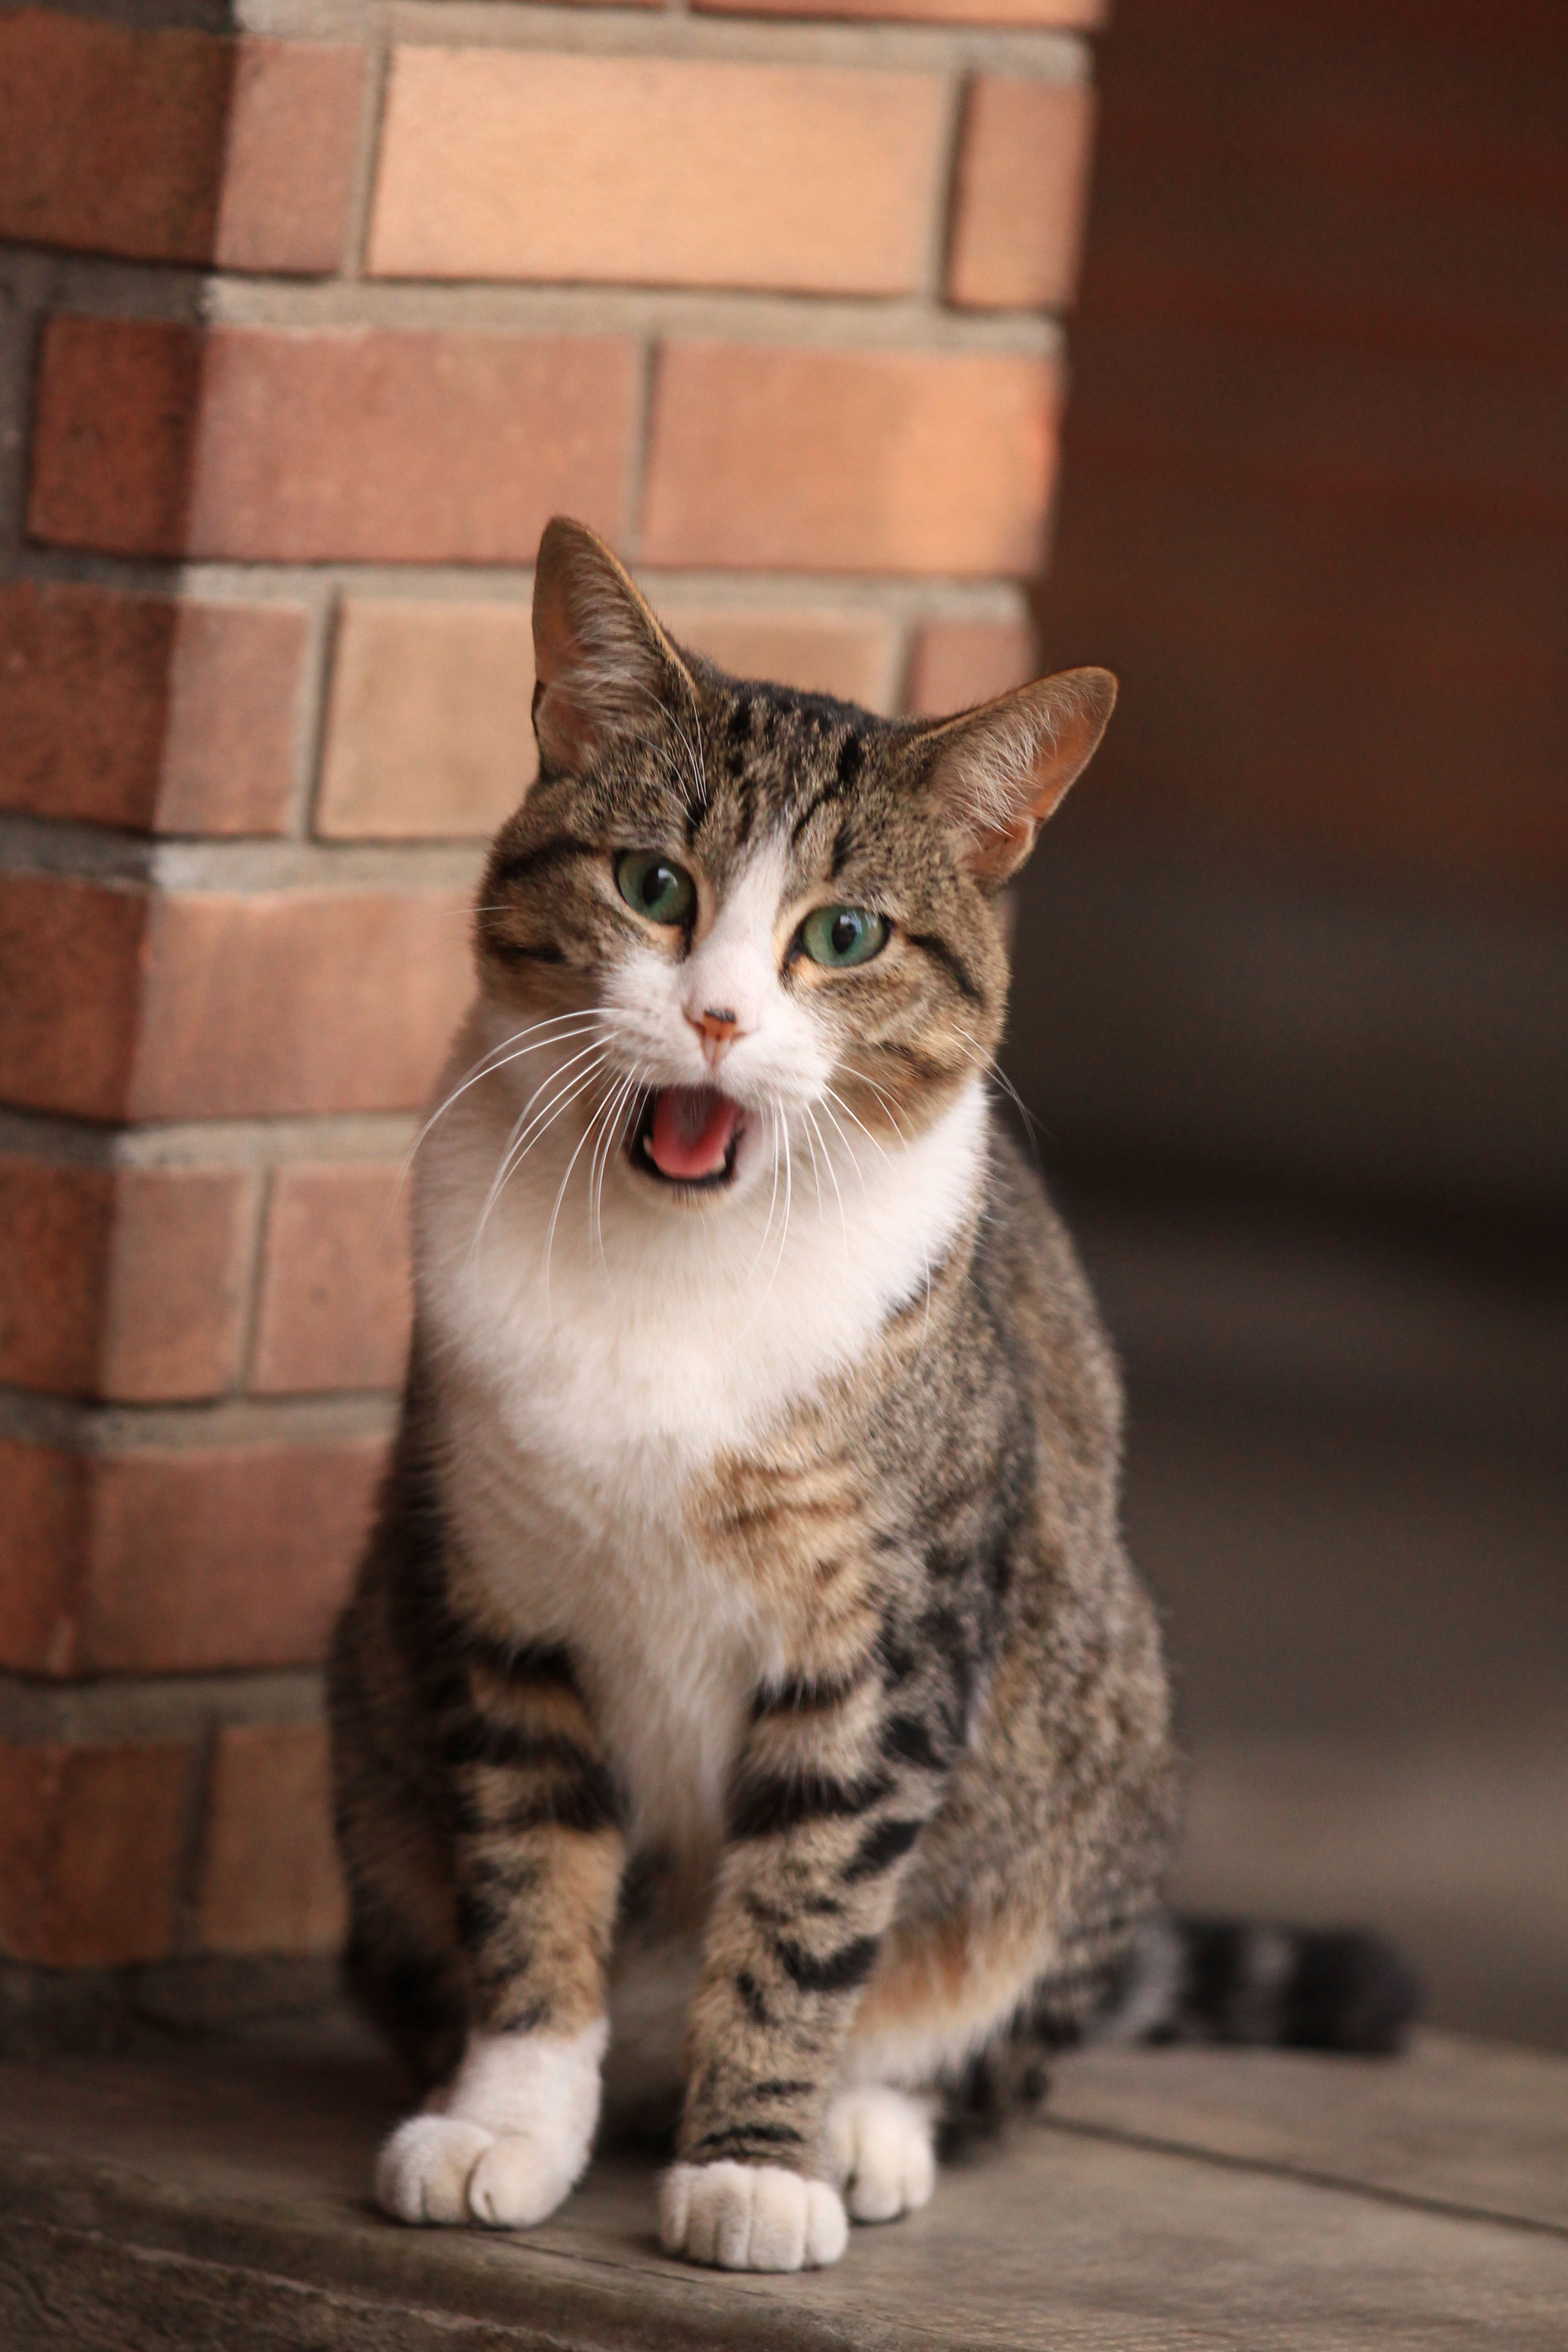
\includegraphics[width=0.3\textwidth]{./Bilder/European_cat_02_16_mp.jpg}
\caption{Example picture for the experiments \cite{cat}}
\label{fig:cat}
\end{figure}
\paragraph{Batch Size}
%%mathe defs of throughput?
Batch Size denotes the number of images fed into the deep learning model in a single inference operation. 
Feeding more than one image to the network can lead to a higher throughput, if enough computational power is available. This increase in throughput often comes at the cost of increased latency and general resource consumption.

To study these trade-offs we conduct experiments with the following batch sizes: 1, 2, 16, 32. Since at the point of these experiments a batch size greater than one is not supported for the TensorFlow Lite versions of MobilenetV2 (both float and quantized), measurements with these batch sizes cannot be performed for the case of edge inference at this point.
\paragraph{NNAPI}
The Android Neural Network API (NNAPI), presented in section \ref{chap:NNAPI}, is supposed to enhance the inference performance of TensorFlow Lite. Therefore we take a look into the effect of this framework.
%%Mention GPU use here
\paragraph{GPU Usage}
Since January 16 an experimental release of TensorFlow Lite supporting GPU usage on Android using OpenGL ES 3.1 Compute Shaders \cite{tfLiteGPU}.
So far only four public models and their operators are supported, including MobileNetV2, but not InceptionV4. 
Therefore we omit the test of this new feature in our experimentation, but our initial testing indicated that the use of NNAPI provides faster inference latencies for MobileNetV2 than the GPU version.
%%https://medium.com/tensorflow/tensorflow-lite-now-faster-with-mobile-gpus-developer-preview-e15797e6dee7
%experimental
%only mobilenet supported
%worse performance than NNAPI so far
\paragraph{Preprocessing Mode}
For the case of cloud inference the major parts of the needed preprocessing is either done on the edge before sending the image to the cloud or done on cloud.
\paragraph{Inference Mode}
The inference can either be performed on the edge or an a cloud-backend.


\begin{figure}[H]
\centering
 \scalebox{.7}{%\documentclass[border=10pt]{standalone}
%\usepackage{tikz}
%\begin{document}
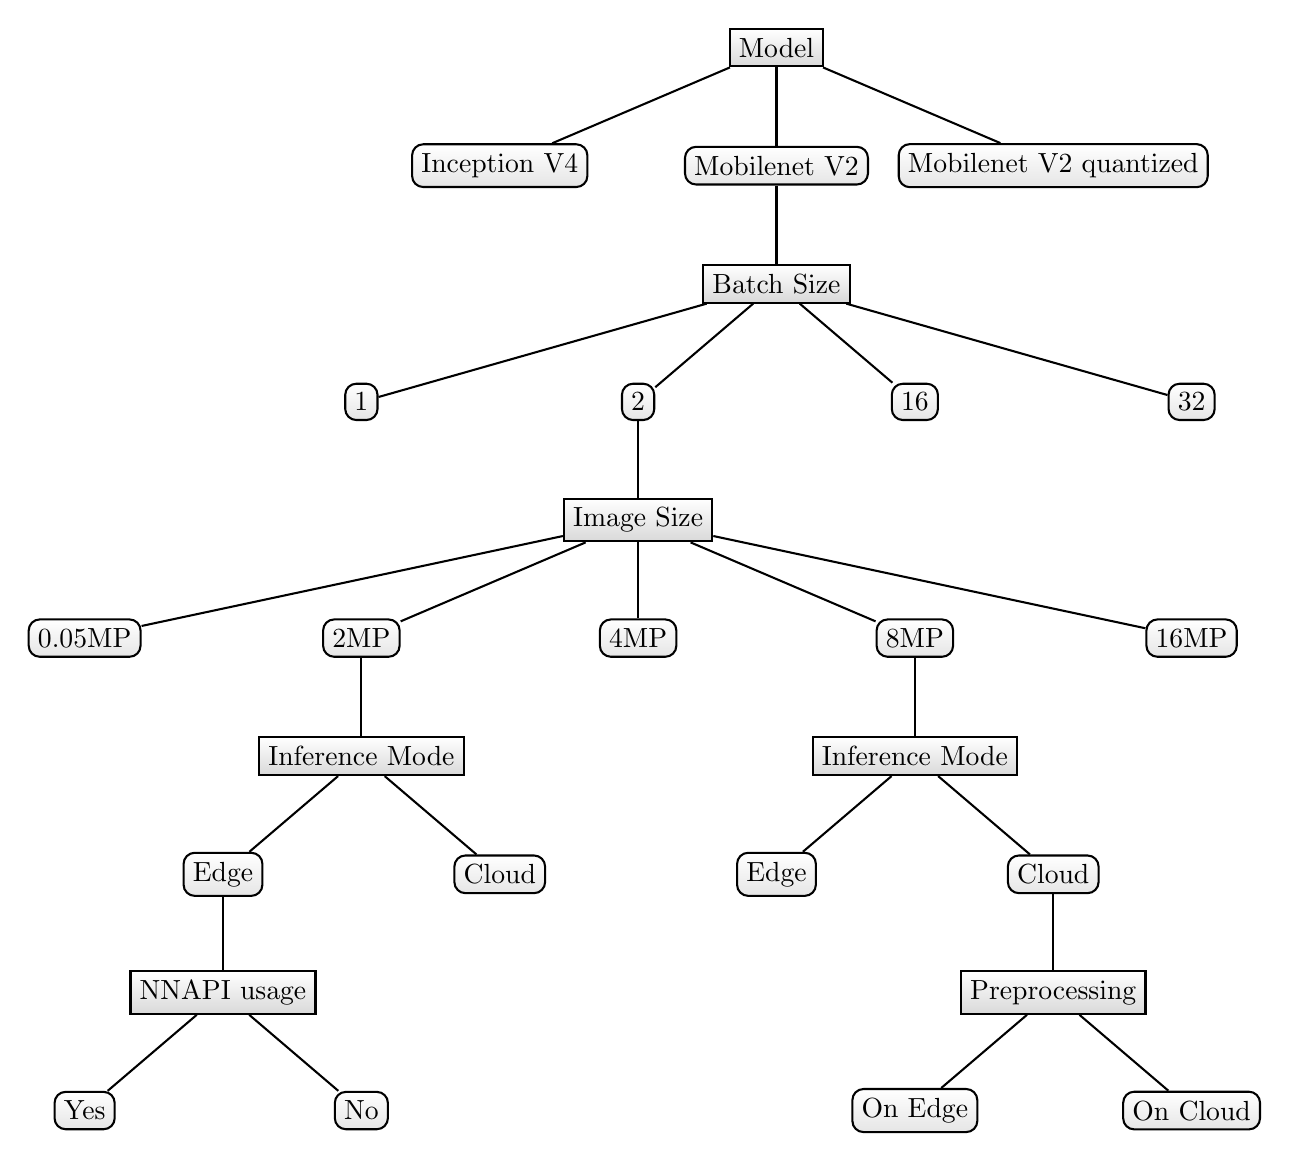
\begin{tikzpicture}[sibling distance=10em,
  param/.style={shape=rectangle,
    draw, align=center,
    top color=white, bottom color=gray!30},
  conf/.style={shape=rectangle, rounded corners,
    draw, align=center,
    top color=white, bottom color=gray!20}  ]  ]
    
  \node[param] {Model}
    child { node [conf]{Inception V4} }
    child { node [conf]{Mobilenet V2}
      child { node [param]{Batch Size}
        child { node [conf]{1} }
        child { node [conf]{2} 
            child { node [param]{Image Size}
                child { node [conf]{0.05MP}}
                child { node [conf]{2MP}
                child { node [param]{Inference Mode}
                        child { node[conf] {Edge}
                            child { node[param] {NNAPI usage}
                                 child { node[conf] {Yes}}
                                 child { node [conf]{No}}}}
                        child { node [conf]{Cloud}
                            }}}
                child { node [conf]{4MP}
                    }
                child { node [conf]{8MP}
                child { node [param]{Inference Mode}
                        child { node[conf] {Edge}}
                        child { node [conf]{Cloud}
                            child { node [param]{Preprocessing}
                               child { node [conf]{On Edge}}
                                child { node [conf]{On Cloud}}}}}}
                child { node [conf]{16MP}}}}
        child { node[conf] {16} }
        child { node [conf]{32} }} }
    child { node [conf]{Mobilenet V2 quantized} };
\end{tikzpicture}
%\end{document}}

\caption{Excerpt of the performed experiments configurations}
\label{fig:tree}
\end{figure}
Figure \ref{fig:tree} shows a part of our experimentation tree. In theory there would be 240 different parameter configurations, but due to a number of reasons the number of different configurations reduced to 113 in total.

First, the Usage of NNAPI is independent of the image size hence we only perform experiments without NNAPI for a single Image Size. Also the usage of NNAPI leads to a way better performance for edge inference and we want to compare edge and cloud inference so we only carry out experiments without NNAPI for a batch size of one.
We omit the cloud inference for the quantized MobileNetV2 because the model is so small the network overhead would be overwhelming.%INSERT REASON.

%of limited capacity/time and
Lastly due to lack of support of batch sizes larger than one in TensorFlow Lite for the MobileNet models.
\subsection{Performance Metrics}
\label{chap:insta_measurements}
We conduct the measurements either directly in the source code or by using Android Studio Profiler (Version 3.3). Since Android Studio cannot collect all metrics the way we wanted, we wanted to used Trepn as a secondary profiling application. But since Trepn does not support our test device, we had to omit these metrics.

In the following definitions $t_{start}$ denotes the starting point of either the preprocessing or inference, while $t_{end}$ denotes the end point of the respective process.
\subsubsection{Latency}
We measure $Latency_{preprocessing}$ by measuring the time difference between start and end of the preprocessing process.
Note that all latency measurements are reported in milliseconds(ms).
\begin{equation*}
\begin{gathered}
Latency_{preprocessing} = t_{end} - t_{start}
\end{gathered}
\end{equation*}
To measure inference latency we need to distinguish between edge and cloud inference, since for the latter the network latency needs to be considered.

\paragraph{Edge Inference}To measure edge inference latency we measure the time the TensorFlow Lite interpreter needs to run the inference operation on the loaded model given the input image.
\begin{equation*}
\begin{gathered}
Latency_{inference} = t_{end} - t_{start}
\end{gathered}
\end{equation*}
\paragraph{Cloud Inference}
To measure the cloud inference latency we need to measure two latencies, which combined yield $Latency_{inference}$. The first latency is  $Latency_{server}$. This server latency describes the time difference between the point where TensorFlow Serving receives the inference request and the point in time where TensorFlow Serving sends the response back to the client.
The second latency $Latency_{network}$ denotes the time the prediction request needs to reach the cloud-backend.
These latencies are illustrated in figure \ref{fig:serverLat}.
\begin{figure}[!htb]
\centering


\tikzset{every picture/.style={line width=0.75pt}} %set default line width to 0.75pt        

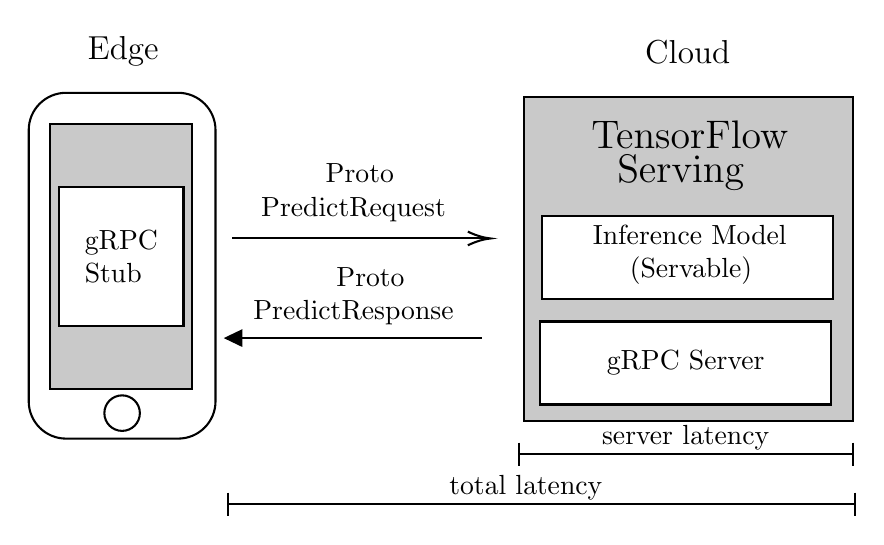
\begin{tikzpicture}[x=0.75pt,y=0.75pt,yscale=-1,xscale=1]
%uncomment if require: \path (0,300); %set diagram left start at 0, and has height of 300

%Straight Lines [id:da7072764839644827] 
\draw    (149.5,277) -- (451.5,277) ;
\draw [shift={(451.5,277)}, rotate = 180] [color={rgb, 255:red, 0; green, 0; blue, 0 }  ][line width=0.75]    (0,5.59) -- (0,-5.59)   ;
\draw [shift={(149.5,277)}, rotate = 180] [color={rgb, 255:red, 0; green, 0; blue, 0 }  ][line width=0.75]    (0,5.59) -- (0,-5.59)   ;
%Straight Lines [id:da9536138531960994] 
\draw    (289.5,253) -- (450.5,253) ;
\draw [shift={(450.5,253)}, rotate = 180] [color={rgb, 255:red, 0; green, 0; blue, 0 }  ][line width=0.75]    (0,5.59) -- (0,-5.59)   ;
\draw [shift={(289.5,253)}, rotate = 180] [color={rgb, 255:red, 0; green, 0; blue, 0 }  ][line width=0.75]    (0,5.59) -- (0,-5.59)   ;
%Shape: Rectangle [id:dp8902536871651789] 
\draw  [fill={rgb, 255:red, 201; green, 201; blue, 201 }  ,fill opacity=1 ] (63.91,93.69) -- (132.34,93.69) -- (132.34,221.63) -- (63.91,221.63) -- cycle ;
%Rounded Rect [id:dp41557214204551274] 
\draw   (53.5,96.82) .. controls (53.5,86.88) and (61.56,78.82) .. (71.5,78.82) -- (125.5,78.82) .. controls (135.44,78.82) and (143.5,86.88) .. (143.5,96.82) -- (143.5,227.43) .. controls (143.5,237.37) and (135.44,245.43) .. (125.5,245.43) -- (71.5,245.43) .. controls (61.56,245.43) and (53.5,237.37) .. (53.5,227.43) -- cycle ;
%Shape: Ellipse [id:dp8878397246816687] 
\draw   (89.95,233.16) .. controls (89.95,228.43) and (93.78,224.6) .. (98.5,224.6) .. controls (103.22,224.6) and (107.05,228.43) .. (107.05,233.16) .. controls (107.05,237.88) and (103.22,241.71) .. (98.5,241.71) .. controls (93.78,241.71) and (89.95,237.88) .. (89.95,233.16) -- cycle ;
%Straight Lines [id:da5813802620369573] 
\draw    (151.48,149) -- (274,149) ;
\draw [shift={(276,149)}, rotate = 540] [color={rgb, 255:red, 0; green, 0; blue, 0 }  ][line width=0.75]    (10.93,-3.29) .. controls (6.95,-1.4) and (3.31,-0.3) .. (0,0) .. controls (3.31,0.3) and (6.95,1.4) .. (10.93,3.29)   ;

%Straight Lines [id:da16220168680973557] 
\draw    (149.48,197) -- (272,197) ;

\draw [shift={(147.48,197)}, rotate = 360] [fill={rgb, 255:red, 0; green, 0; blue, 0 }  ][line width=0.75]  [draw opacity=0] (8.93,-4.29) -- (0,0) -- (8.93,4.29) -- cycle    ;
%Shape: Rectangle [id:dp8411150472244695] 
\draw  [fill={rgb, 255:red, 201; green, 201; blue, 201 }  ,fill opacity=1 ] (292,81) -- (450.5,81) -- (450.5,237) -- (292,237) -- cycle ;
%Shape: Rectangle [id:dp13557861576626729] 
\draw  [fill={rgb, 255:red, 255; green, 255; blue, 255 }  ,fill opacity=1 ] (301,138) -- (441,138) -- (441,178) -- (301,178) -- cycle ;
%Shape: Rectangle [id:dp5681963435258506] 
\draw  [fill={rgb, 255:red, 255; green, 255; blue, 255 }  ,fill opacity=1 ] (68.19,124.22) -- (128.07,124.22) -- (128.07,191.1) -- (68.19,191.1) -- cycle ;
%Shape: Rectangle [id:dp7458124222136935] 
\draw  [fill={rgb, 255:red, 255; green, 255; blue, 255 }  ,fill opacity=1 ] (300,189) -- (440,189) -- (440,229) -- (300,229) -- cycle ;

% Text Node
\draw (370,245) node  [align=left] {server latency};
% Text Node
\draw (293,269) node  [align=left] {total latency};
% Text Node
\draw (210,127) node  [align=left] { \ \ \ \ \ \ \ Proto\\PredictRequest};
% Text Node
\draw (99,59) node  [align=left] {{\large Edge}};
% Text Node
\draw (371,59) node  [align=left] {{\large Cloud}};
% Text Node
\draw (372,109) node  [align=left] {{\Large TensorFlow}\\{\Large  \ \ Serving}};
% Text Node
\draw (372,157) node  [align=left] {Inference Model\\ \ \ \ \ (Servable)};
% Text Node
\draw (210,177) node  [align=left] { \ \ \ \ \ \ \ \ \ Proto\\PredictResponse};
% Text Node
\draw (98.13,157.66) node  [align=left] {gRPC\\ Stub};
% Text Node
\draw (370,209) node  [align=left] {gRPC Server};


\end{tikzpicture}
\caption{Measurement of $Latency_{server}$ and $Latency_{network}$ for Cloud Inference}
\label{fig:serverLat}
\end{figure}


Similar to the edge inference, $Latency_{inference}$ is being measured by calculating the time difference between starting the inference process and receiving the prediction for the given inference request. This whole process is covered by the \emph{predict} function of TensorFlow Serving. Therefore we measure the wall clock time of this function.

Since TensorFlow Serving does not output the server latency, we needed to tweak the source code of gRPC, which is the underlying protocol of TensorFlow Serving. gRPC already logs this latency, so we adjust the source code to output this latency when a call to TensorFlow Serving is finished, repackage the source code and change to dependencies of TensorFlow Serving pointing to the adjusted packages.

We then calculate $Latency_{network}$ implicitly by subtracting $Latency_{server}$ from $Latency_{inference}$.

\begin{equation*}
\begin{gathered}
Latency_{inference} = t_{end} - t_{start}\\
Latency_{server}= t_{receive Request} - t_{send Response}\\
Latency_{network} = Latency_{inference} - Latency_{server}
\end{gathered}
\end{equation*}


The total latency $Latency_{total}$ for both edge and cloud inference is simply calculated by summing up the latencies of both preprocessing and inference.
\begin{equation*}
\begin{gathered}
Latency_{total} = Latency_{preprocessing} + Latency_{inference}
\end{gathered}
\end{equation*}
\subsubsection{Energy Consumption}
Since Android Studio Profiler only estimates the energy consumption in the form of low, medium and high, the tool is not fit to provide empiric measurements. The Trepn Power Profiler would provide such measurements, but does not support the device used for the experiments (OnePlus 6T).
\subsubsection{CPU Usage}
We measure the CPU usage(\%) of both preprocessing as the maximum CPU usage during the respective processes.
\begin{equation*}
\begin{gathered}
%%CPU_{preprocessing} = max_{[start_{preprocessing}, end_{preprocessing}]}(CPU)\\
%%CPU_{inference} = max_{[start_{inference}, end_{inference}]}(CPU)\\
CPU_{preprocessing} = \max\limits_{t_{start} \leq t \leq t_{end}} CPU_{Usage}(t)\\
CPU_{inference} = \max\limits_{t_{start} \leq t \leq t_{end}} CPU_{Usage}(t)
\end{gathered}
\end{equation*}
Android Studios’ CPU Profiler allows us to record the maximum CPU usage for both preprocessing and inference. To minimize the impact on the Android Profiler on the performance of the application we disable allocation tracking.
\begin{figure}[H]
\centering  
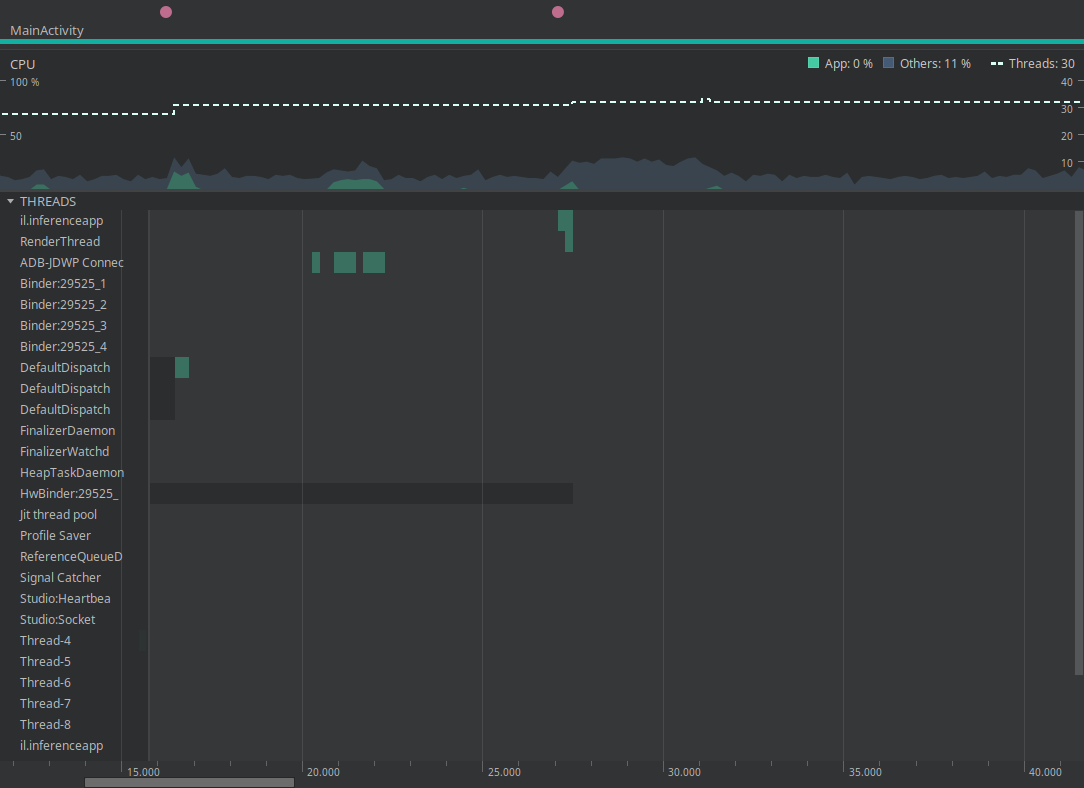
\includegraphics[width=0.6\textwidth]{./Bilder/profiler_CPU}
\caption{Android CPU Profiler}
\label{fig:prof_cpu}
\end{figure}
\subsubsection{Memory Usage}
We measure the memory usage by recording the maximum memory consumption during both processing and inference. Both of the following metrics are reported in megabytes(MB) in the result section.
\begin{equation*}
\begin{gathered}
Memory_{preprocessing} = \max\limits_{t_{start} \leq t \leq t_{end}} Memory(t)\\\\
Memory_{inference} = \max\limits_{t_{start} \leq t \leq t_{end}} Memory(t)\\
\end{gathered}
\end{equation*}
The Memory Profiler is part of Android Studio Profiler and shows the memory consumption of the app it is profiling. Memory allocations by the operating system or other apps are not recorded. Besides recording the total amount of memory allocated the Profiler also tracks the different categories, for example memory allocated by Java/Kotlin code. We always record the maximum consumed memory for each operation.

Figure \ref{fig:prof_mem} depicts an example of the Memory Profiler for a single experiment. The first peak in memory consumption is the preprocessing step, while the second peak is caused by the inference process.
The little trash can at the bottom of the figure shows that the garbage collection was called. The garbage collection was always manually called after the preprocessing in case not all unneeded memory allocations are collected before running the inference operation. 
Note that we report total memory consumption of the application, including memory consumed for the graphical interface or the \emph{Logger} class.
%In the case of preprocessing only the preprocessed image is needed, so the 
\begin{figure}[H]
\centering
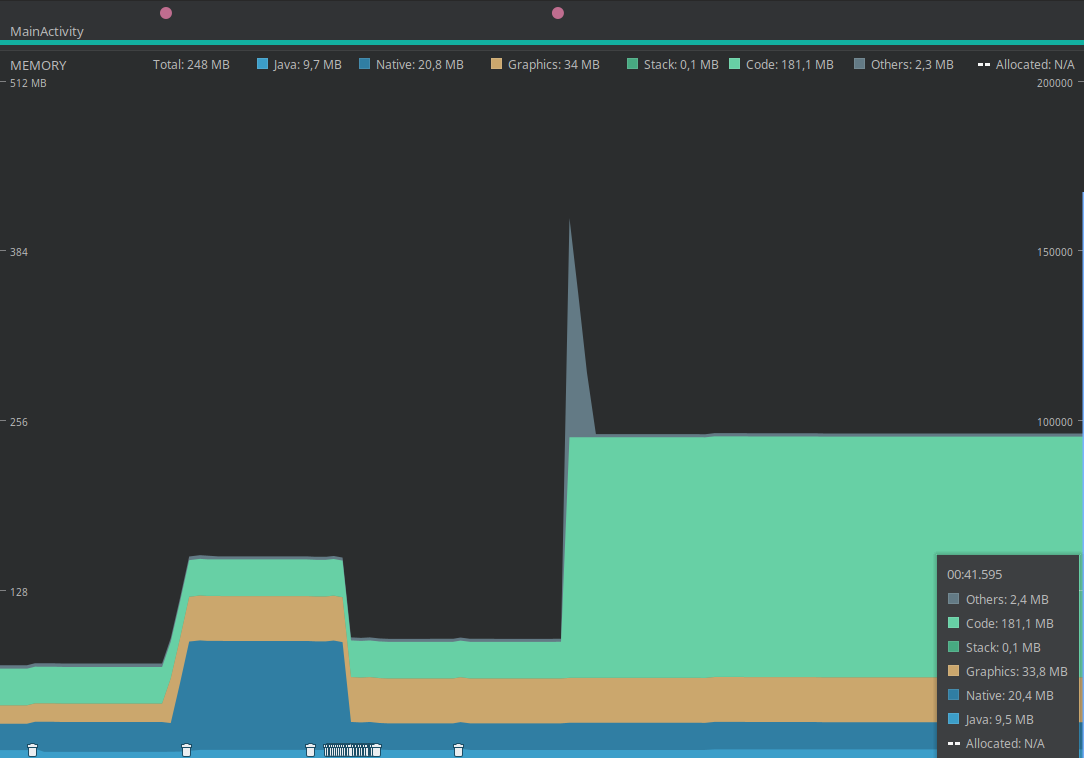
\includegraphics[width=0.6\textwidth]{./Bilder/profiler_MEM}
\caption{Android Memory Profiler}
\label{fig:prof_mem}
\end{figure}
\subsubsection{GPU Usage}
Neither Android Studio nor Trepn can provide GPU metrics for the OnePlus 6T. Hence no GPU measurements can be conducted.
\subsubsection{Throughput}
We differentiate three types of throughput: the inference throughput, preprocessing throughput and the total throughput, which also includes preprocessing besides inference.
We calculate throughput in operations per second by 

\begin{equation*}
\begin{gathered}
Throughput_{preprocessing} =\frac{1000}{(Latency_{preprocessing}) / batchsize}\\
Throughput_{inference} =\frac{1000}{(Latency_{inference}) / batchsize}\\
Throughput_{total}  =\frac{1000}{(Latency_{total}) / batchsize}
\end{gathered}
\end{equation*}
\subsubsection{Data Consumption}
We measure both transmitted and received data by using the Android TrafficStats package (https://developer.android.com/reference/android/net/TrafficStats). We start measuring both transmitted and received bytes when the inference operation is started and stop when the response from the server is returned. We report both $Data_{transmitted}$ and $Data_{received}$ in kilobytes(KB).
\begin{equation*}
\begin{gathered}
Data_{transmitted} = \sum_{t_{start}}^{t_{end}} Data_{transmitted}(t)\\
Data_{received} = \sum_{t_{start}}^{t_{end}} Data_{received}(t)
\end{gathered}
\end{equation*}
\section{Results and Evaluation}
This section covers the results of the conducted experiments and their evaluation.

First, we take a look into the individual results of edge and cloud inference and afterwards compare them against each other. In each of these sections first the preprocessing and then the inference results are presented.
%die 83mb aufschlüsseln in GUI etc 
Note that the Android application consumed around 83MB in memory and 0\% CPU during idle.

For precise mean values and standard deviations of all measured metrics refer to tables \ref{measurementsInception} and \ref{measurementsMobilenet}.

The black bar on top of each bar of the following barchart represents the standard deviation.

Preprocessing is performed without any models loaded and the edge. 
Edge Inference is done using a loaded model. We do not consider model loading time in this thesis.
\subsection{Edge Inference}
This section covers the results of the edge inference experiments with OnePlus 6T device presented in section \ref{chap:hardwareEdge}.
\subsubsection{Preprocessing}
Figure \ref{fig:EdgePrepro} shows the $Latency_{preprocessing}$ and $Memory_{preprocessing}$ for the different image sizes and models.

There is little difference in both latency and memory for the different models. 
InceptionV4 uses more memory than the MobileNet models, which is caused by the models higher input size (InceptionV4 $299\times299$, MobileNetV2 $224\times224$). 

Higher image sizes have an significant impact on the latency as well as memory.
%%factors reinbringen auch kb größe der bilder
%%mehr impact on latency than memory


%%Was über CPU hier sagen
Looking the CPU usages during preprocessing (see figure \ref{fig:CloudEdgePreproCPU}) one can see that the usages are very similar across all models and image sizes. This is probably due to the fact that the preprocessing of a single image is done on a single core.
%%High variance
\begin{figure}[H]
\centering
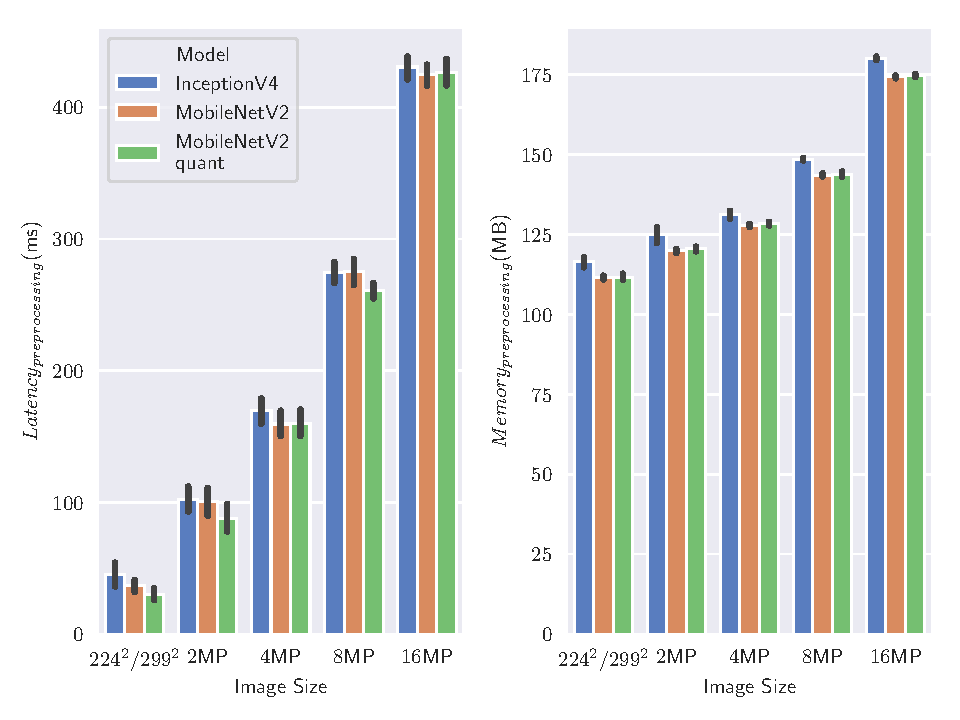
\includegraphics[width=0.8\textwidth]{./Bilder/single_plots/edge_inference_plots/Edge_Inference_Preprocessing.pdf}
\caption{Edge Inference - Preprocessing $Latency_{preprocessing}$, $Memory_{preprocessing}$}
\label{fig:EdgePrepro}
\end{figure}


\subsubsection{Inference}
Different image sizes have no effect on edge inference, as image are always preprocessed when they reach the inference step.
Hence we do not consider the different image sizes in the majority of this section.
\begin{comment}
%%Sagt Grafik was aus?
\begin{figure}[H]
\centering
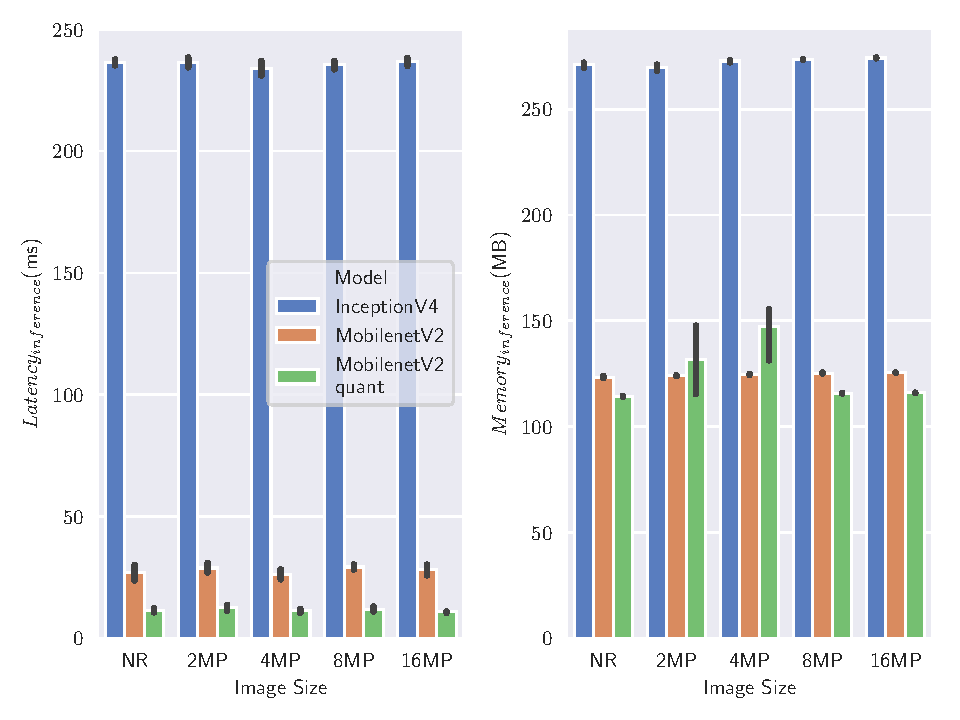
\includegraphics[width=0.8\textwidth]{./Bilder/single_plots/edge_inference_plots/Edge_Inference_Inference.pdf}
\caption{Edge Inference - Inference}
\label{fig:EdgeInference}
\end{figure}


\end{comment}
\subsubsection{Effect of NNAPI}
The Android Neural Network API (NNAPI) is supposed to speed up inference of neural network on Android by introducing optimized kernels/operators. 

The effect of this framework can be seen in figure \ref{fig:NNAPI} and show the significant performance improvement caused by the NNAPI, not only affecting $Latency_{inference}$, but also $Memory_{inference}$ and $CPU_{inference}$.
%%GPU usage ansprechen hier
%%Genauere factors einfügen : inferecen zweimal so schnell...
This effect can be observed across all tested models, but especially on the InceptionV4 network.


Since the NNAPI leads to performance improvements in all measured metrics, it will be used for all further edge inference results.
\begin{figure}[H]
\centering
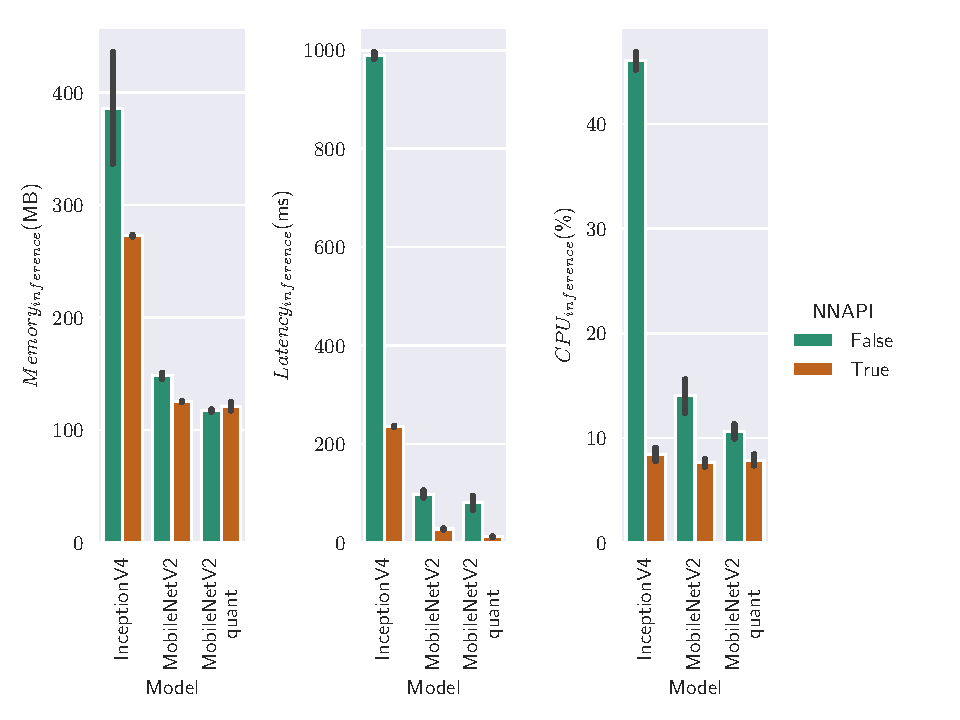
\includegraphics[width=0.9\textwidth]{./Bilder/single_plots/edge_inference_plots/NNAPI_behavior.pdf}
\caption{Edge Inference - Effect of NNAPI on Inference}
\label{fig:NNAPI}
\end{figure}


%%%%%%%%%%%%%%%%%%%%%%%%%%%%%%%%%%%%%%%%%%%%%%%%%%%%%%%%%%%%%%%%%%%
%%%%%Edge Inference Prepro Vs Inference%%%%%%%%%%%%%%%%%%%%%%%%%%%%%%%%%%

Figure \ref{fig:EdgeInferenceRatio} depicts the latency ratio between preprocessing and inference.
As image sizes increases, the preprocessing becomes more and more the bottleneck, especially for the MobileNetV2 models.
For the MobileNetV2 even $224\times224$ images take longer to preprocess than to perform the inference on them.
%The Inception models are far more computational intensive, hence the longer inference latencies, but still 
\begin{figure}[H]
\centering
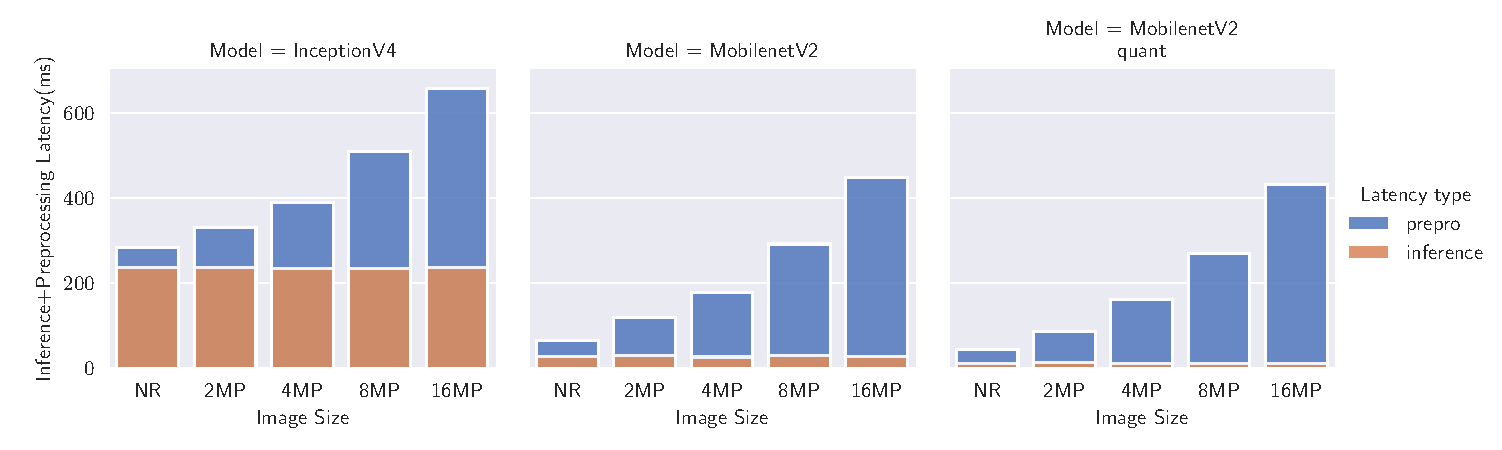
\includegraphics[width=0.95\textwidth]{./Bilder/single_plots/edge_inference_plots/Edge_Preprocessing_+_Inference.pdf}
\caption{Edge Inference - Ratio of Preprocessing and Inference in $Latency_{total}$}
\label{fig:EdgeInferenceRatio}
\end{figure}

\subsection{Cloud Inference}
\subsubsection{Preprocessing}
\begin{figure}[H]


\centering
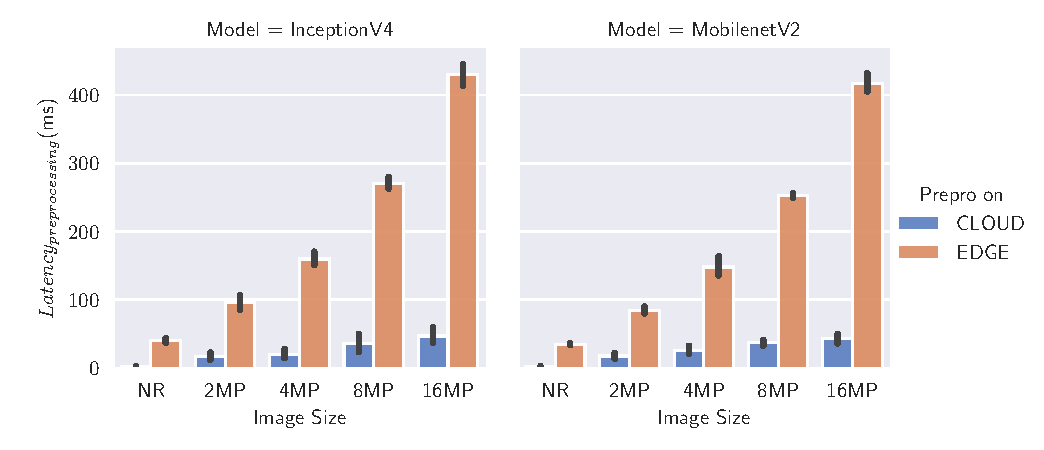
\includegraphics[width=0.95\textwidth]{./Bilder/single_plots/cloud_inference_plots/Cloud_Inference_Preprocessing_Latency.pdf}
\caption{Cloud Inference -  $Latency_{preprocessing}$}
\label{fig:cloudInferencePreproLat}
\end{figure}
\begin{figure}[H]
\centering
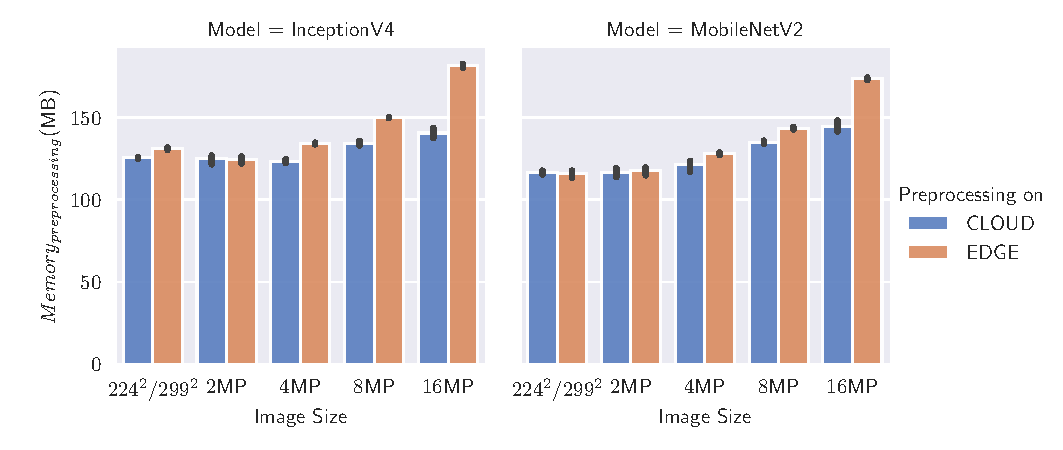
\includegraphics[width=0.95\textwidth]{./Bilder/single_plots/cloud_inference_plots/Cloud_Inference_Preprocessing_Memory.pdf}
\caption{Cloud Inference -  $Memory_{preprocessing}$}
\label{fig:cloudInferencePreproMemory}
\end{figure}
\subsubsection{Inference}
This section focuses on performance differences between the models and the impact of cloud preprocessing on cloud inference.
\begin{figure}[H]
\centering
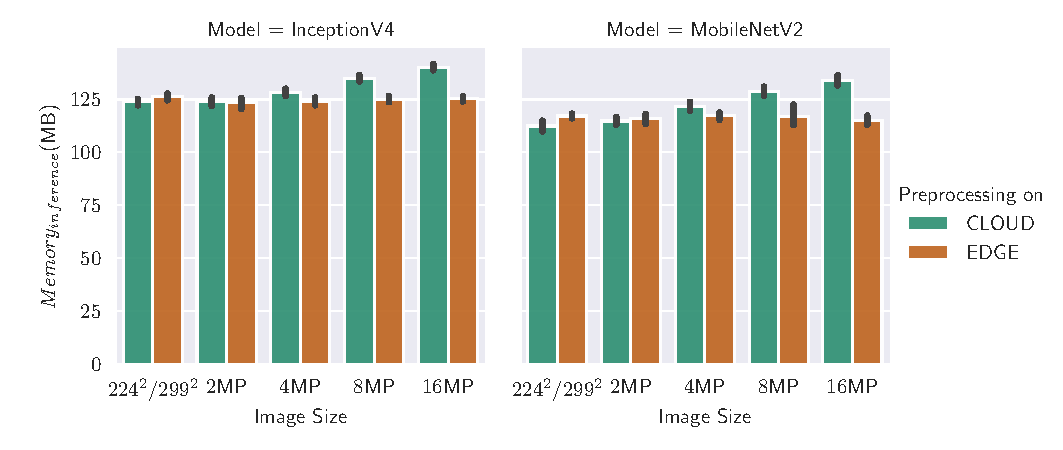
\includegraphics[width=0.95\textwidth]{./Bilder/single_plots/cloud_inference_plots/Cloud_Inference_Memory.pdf}
\caption{Cloud Inference -  $Memory_{inference}$}
\label{fig:cloudInferenceInferenceMemory}
\end{figure}
\begin{figure}[H]
\centering
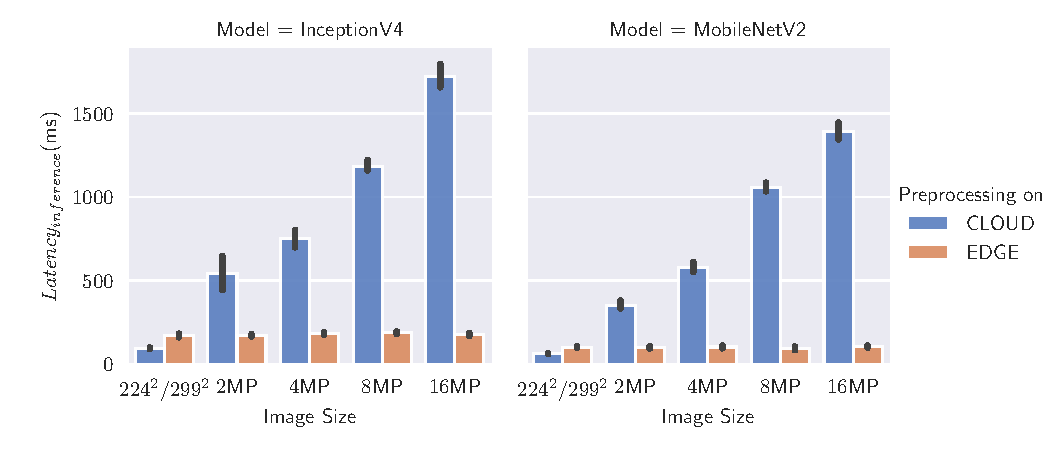
\includegraphics[width=0.95\textwidth]{./Bilder/single_plots/cloud_inference_plots/Cloud_Inference_Latency.pdf}
\caption{Cloud Inference -  $Latency_{inference}$}
\label{fig:cloudInferenceInferenceLatency}
\end{figure}



\begin{figure}[H]
\centering
\begin{subfigure}[b]{0.95\textwidth}
   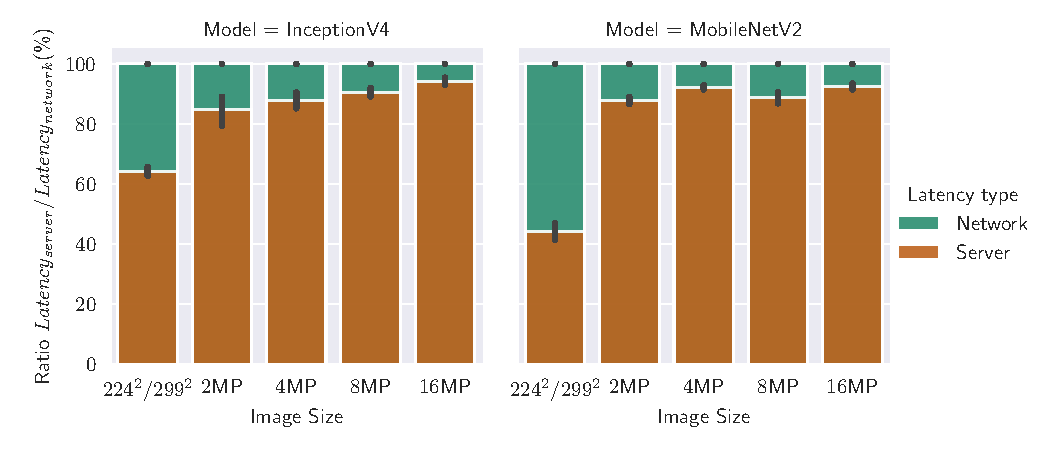
\includegraphics[width=1\linewidth]{./Bilder/single_plots/cloud_inference_plots/Cloud_ratio_server_total_latency_(cloud_prepro).pdf}
   \caption{Cloud Preprocessing}
   \label{fig:CloudInferenceratioCloud} 
\end{subfigure}

\begin{subfigure}[b]{0.95\textwidth}
   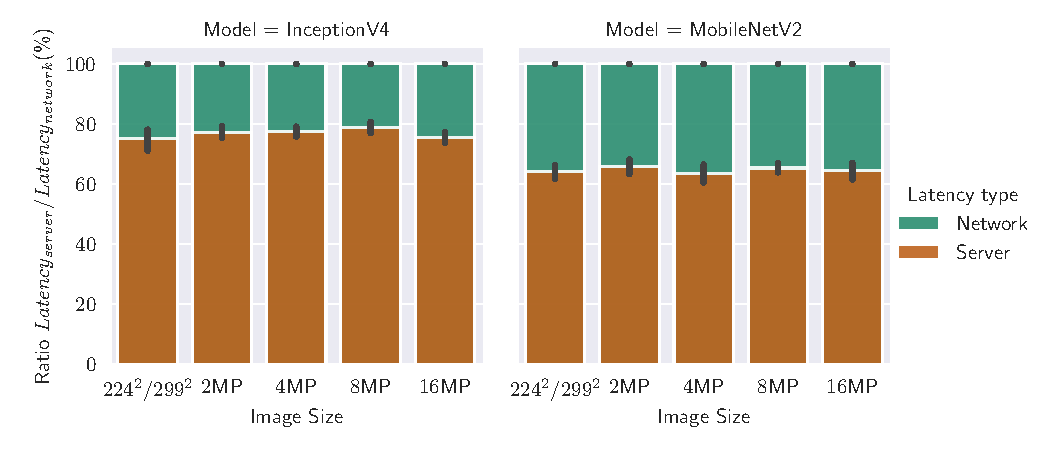
\includegraphics[width=1\linewidth]{./Bilder/single_plots/cloud_inference_plots/Cloud_ratio_server_total_latency_(edge_prepro).pdf}
   \caption{Edge Preprocessing}
   \label{fig:CloudInferenceRatioEdge}
\end{subfigure}

\caption{Cloud Inference -  Ratio between $Latency_{network}$ and $Latency_{server}$}
\end{figure}

\begin{figure}[H]
\centering
\begin{subfigure}[b]{0.95\textwidth}
   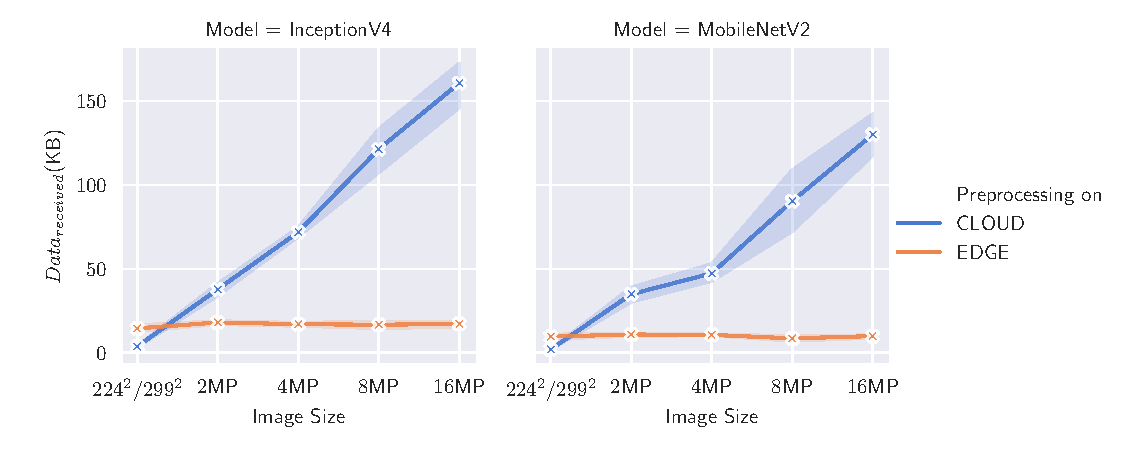
\includegraphics[width=1\linewidth]{./Bilder/single_plots/cloud_inference_plots/Cloud_Inference_Received_Data.pdf}
   \caption{$Data_{received}$}
   \label{fig:CloudInferenceReceivedData} 
\end{subfigure}

\begin{subfigure}[b]{0.95\textwidth}
   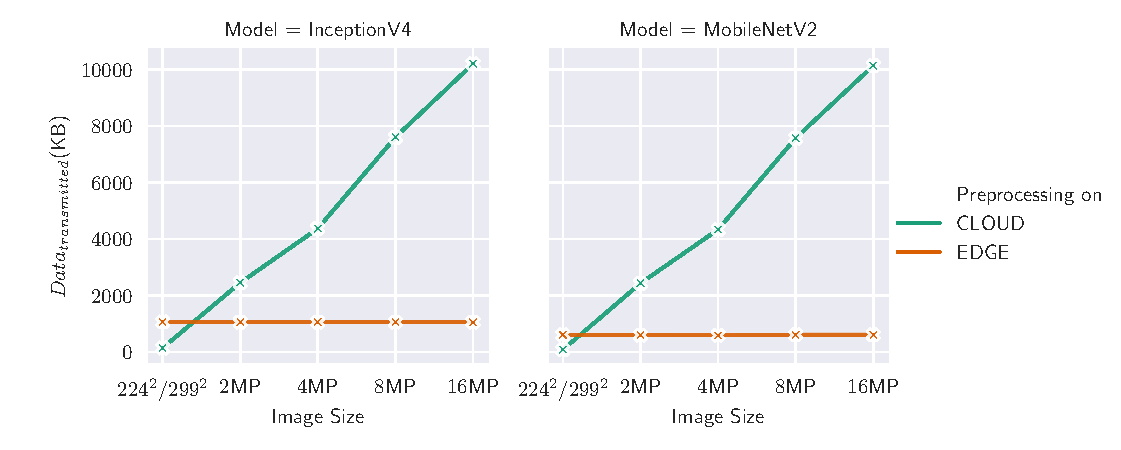
\includegraphics[width=1\linewidth]{./Bilder/single_plots/cloud_inference_plots/Cloud_Inference_Transmitted_Data.pdf}
   \caption{$Data_{transmitted}$}
   \label{fig:CloudInferenceTransmittedData}
\end{subfigure}

\caption{Cloud Inference -  $Data_{received}$ vs. $Data_{transmitted}$}
\end{figure}


\subsection{Edge vs. Cloud Inference}
Now, the results of the cloud and the edge inference are compared against each other.
\subsubsection{Preprocessing}

\begin{figure}[H]
\centering
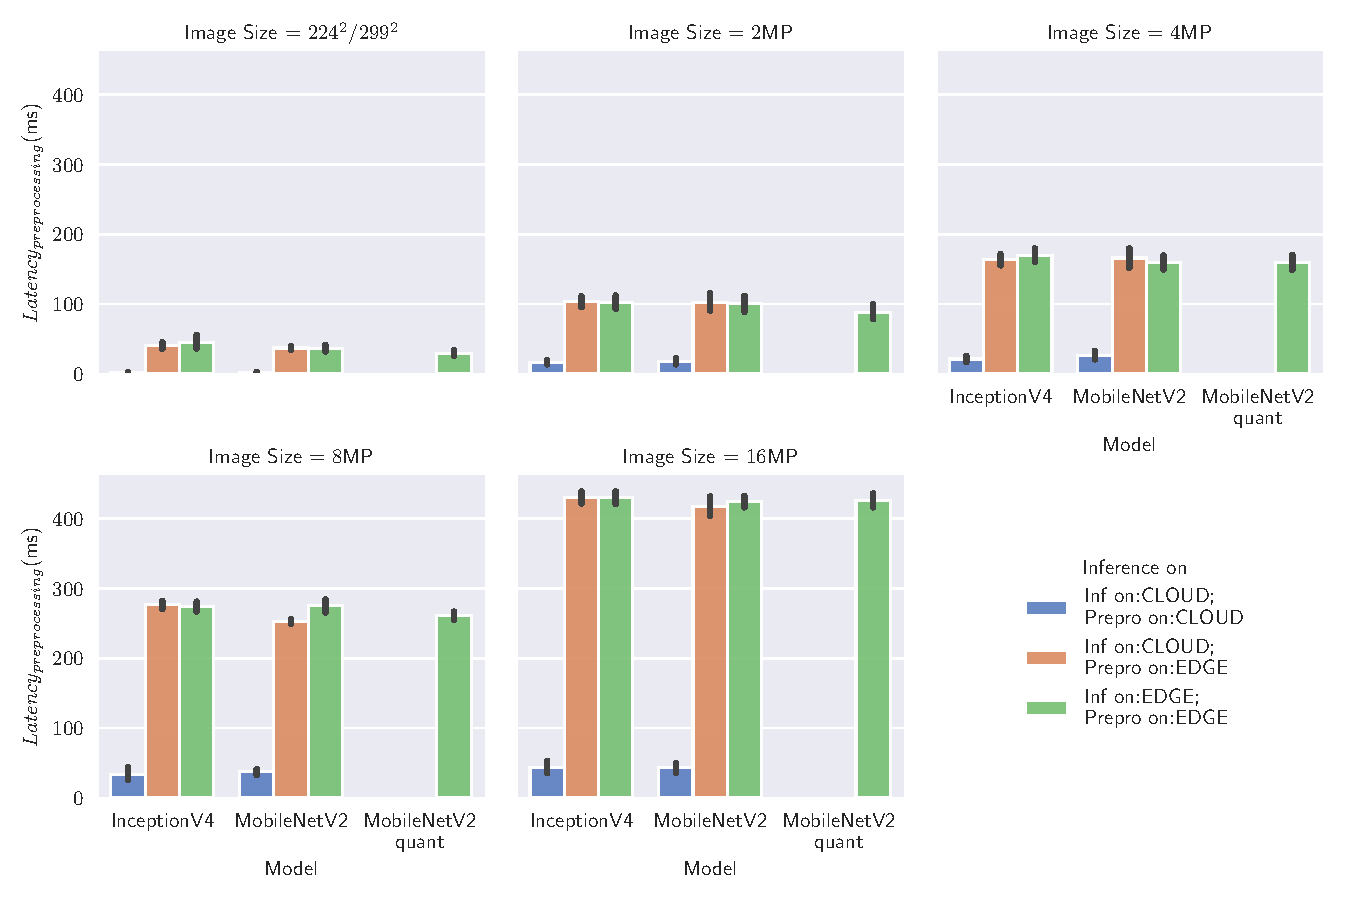
\includegraphics[width=0.95\textwidth]{./Bilder/single_plots/edge_vs_cloud_plots/Edge_vs_Cloud_Inference_Preprocessing_Latencies.pdf}
\caption{Edge vs. Cloud Inference -  $Latency_{preprocessing}$}
\label{fig:EdgeVsCloudPreproLat}
\end{figure}
\begin{figure}[H]
\centering
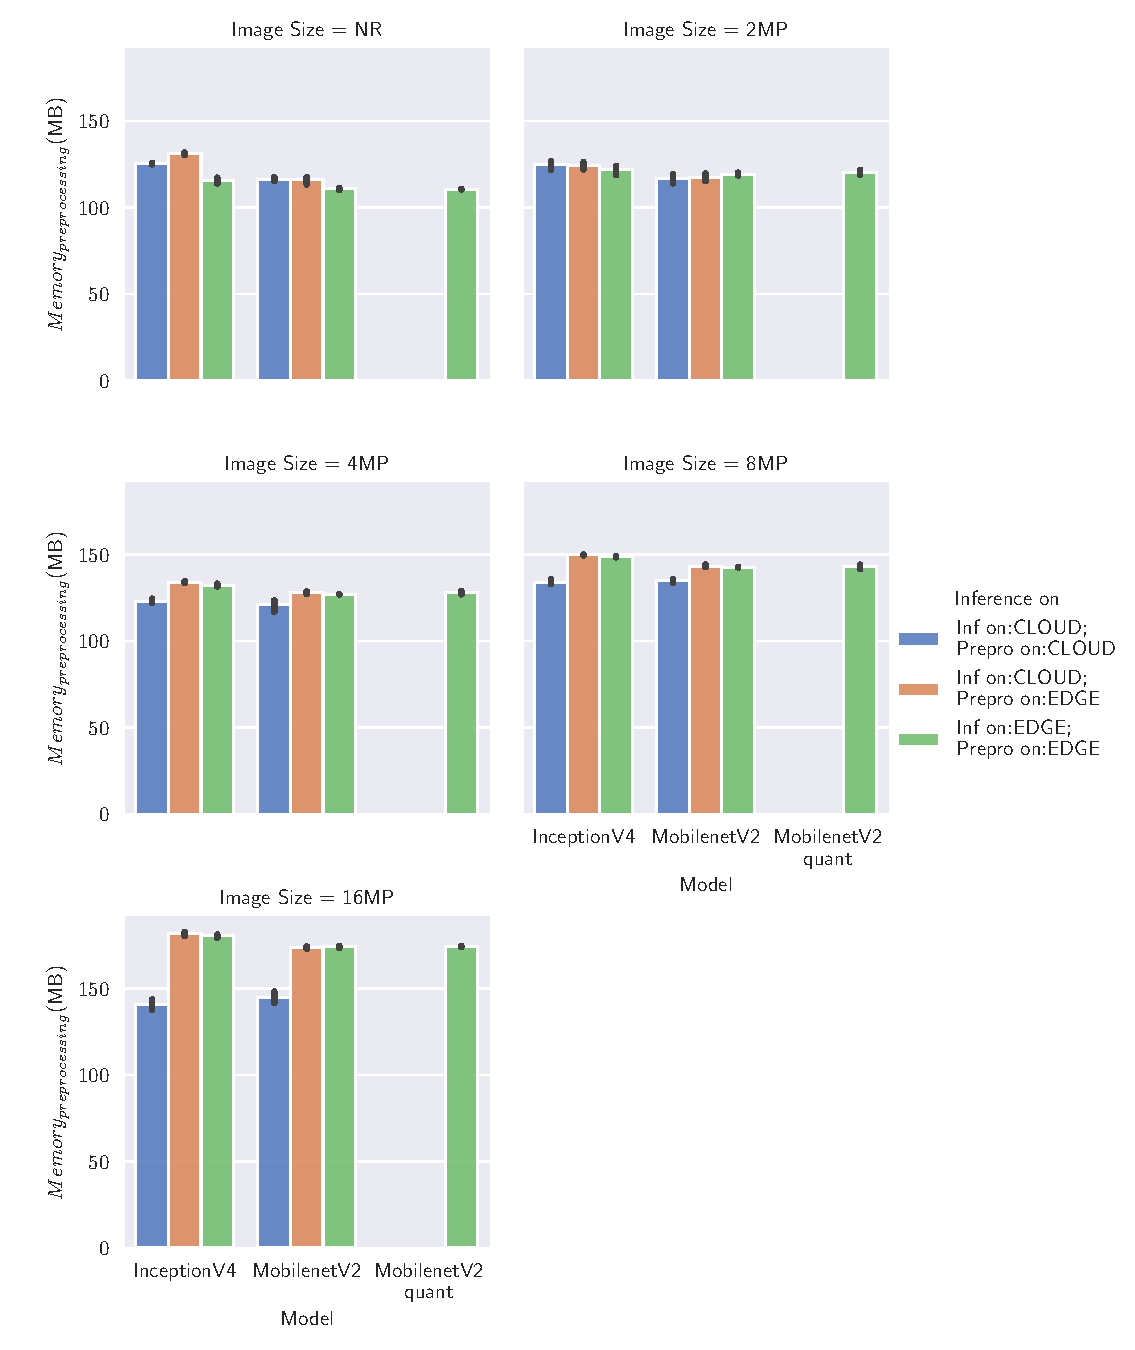
\includegraphics[width=0.95\textwidth]{./Bilder/single_plots/edge_vs_cloud_plots/Edge_vs_Cloud_Inference_Preprocessing_Memory.pdf}
\caption{Edge vs. Cloud Inference -  $Memory_{preprocessing}$}
\label{fig:EdgeVsCloudPreproMemory}
\end{figure}

\subsubsection{Inference}
\begin{figure}[H]
\centering
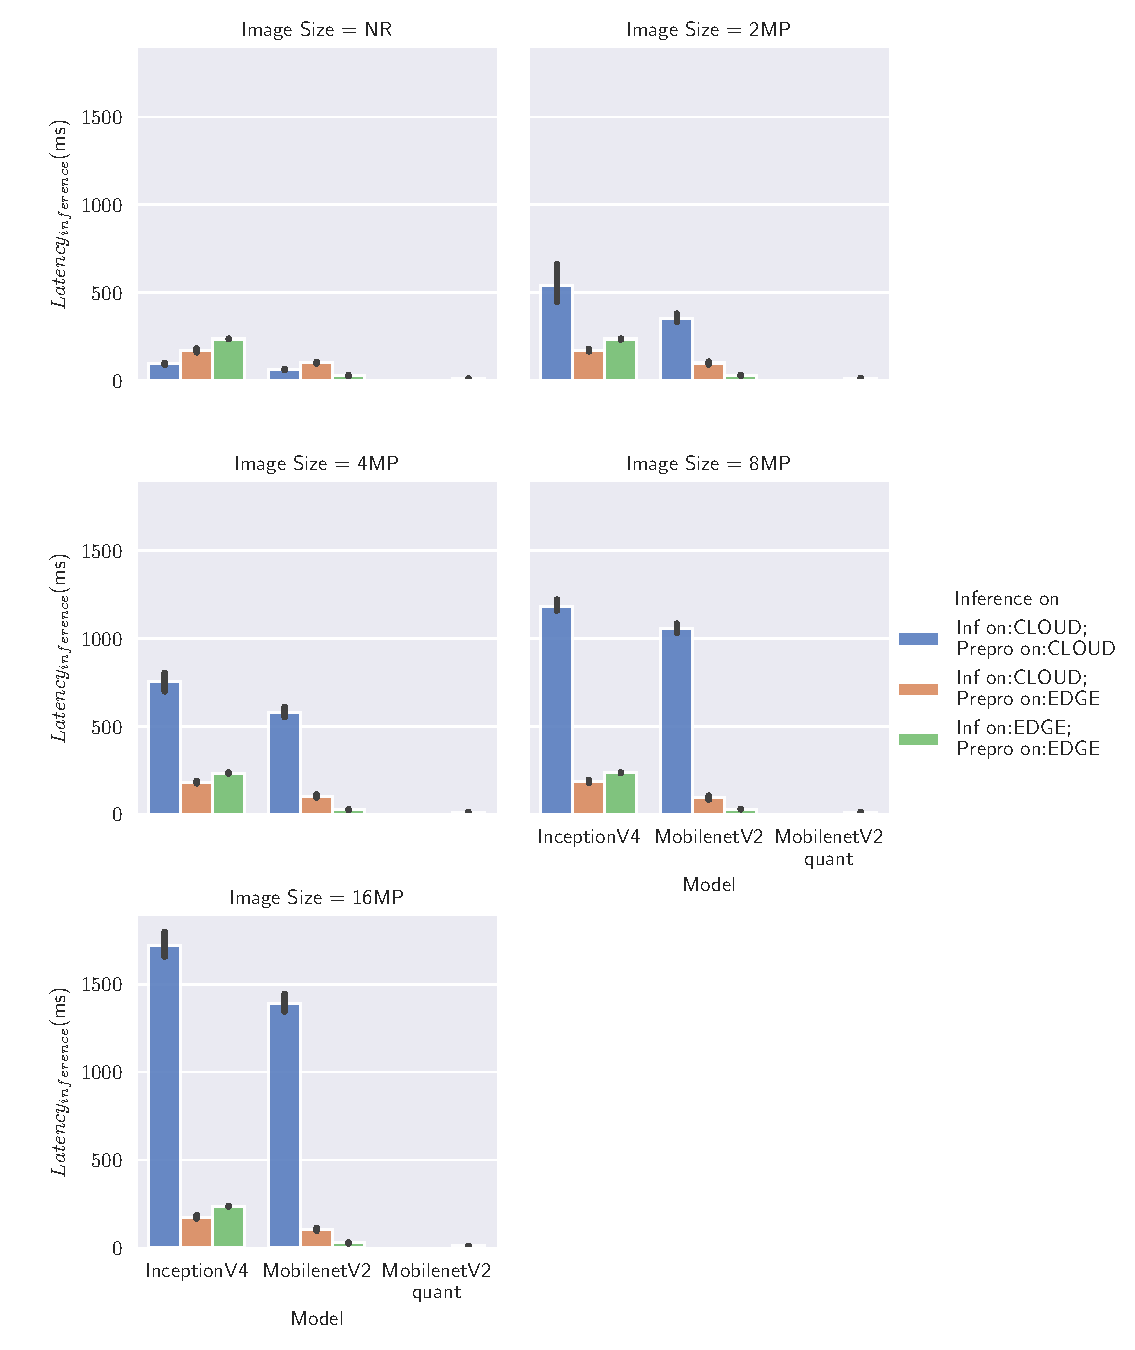
\includegraphics[width=0.95\textwidth]{./Bilder/single_plots/edge_vs_cloud_plots/Edge_vs_Cloud_Inference_Inference_Latencies.pdf}
\caption{Edge vs. Cloud Inference -  $Latency_{inference}$}
\label{fig:EdgeVsCloudInferenceLat}
\end{figure}
\begin{figure}[H]
\centering
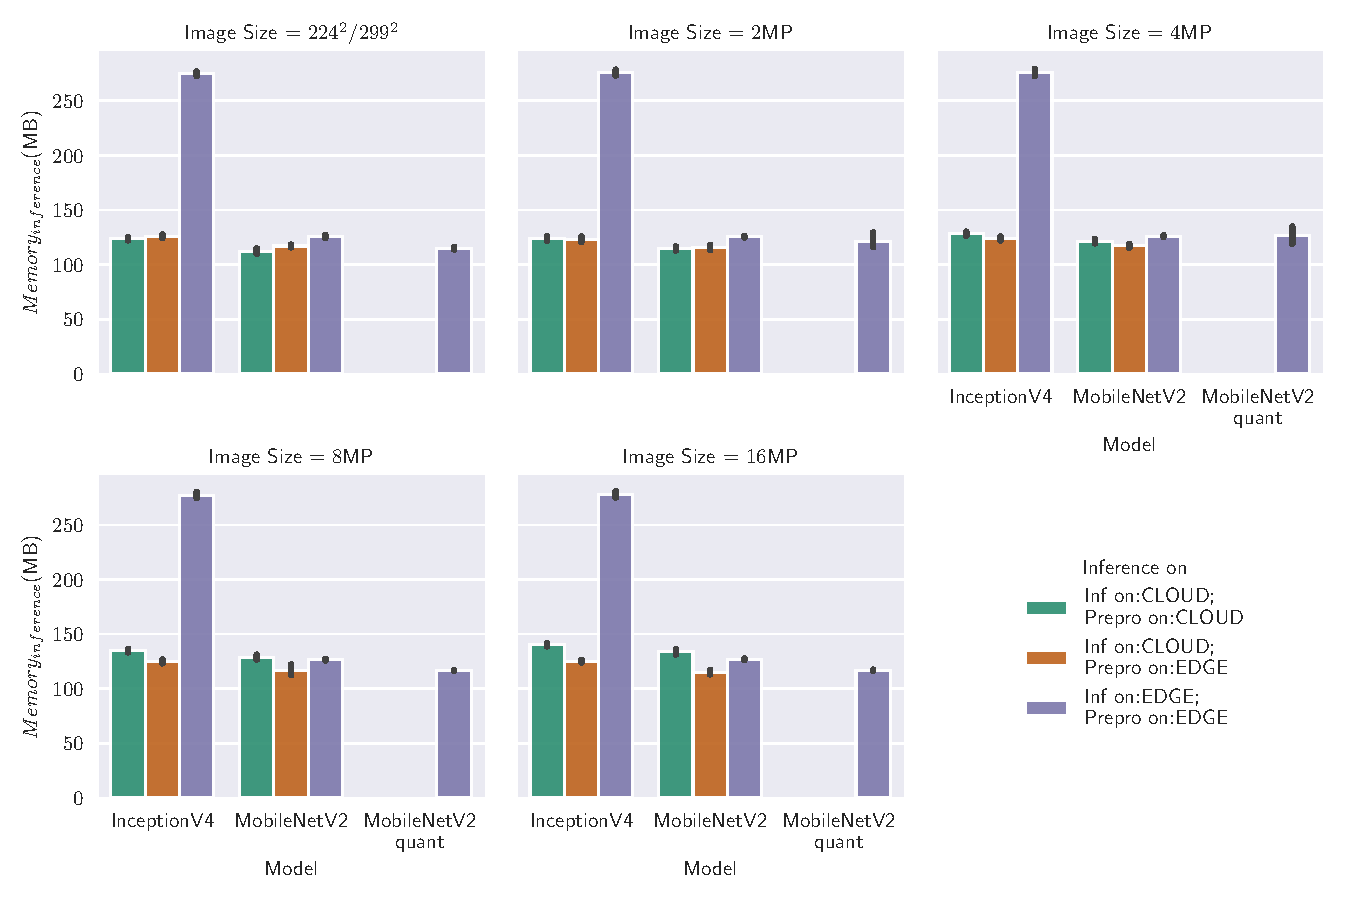
\includegraphics[width=0.95\textwidth]{./Bilder/single_plots/edge_vs_cloud_plots/Edge_vs_Cloud_Inference_Inference_Memory.pdf}
\caption{Edge vs. Cloud Inference -  $Memory_{inference}$}
\label{fig:EdgeVsCloudInferenceMemory}
\end{figure}
\subsection{Effect of larger Batch Sizes}
This section covers the results of the experiments with batch size equal or larger than one. Since the TensorFlow Lite of the used MobileNet version does not allow batch sizes larger than one, edge inference experiments with these models are omitted from this section.
\subsubsection{Preprocessing}
\begin{figure}[H]
\centering
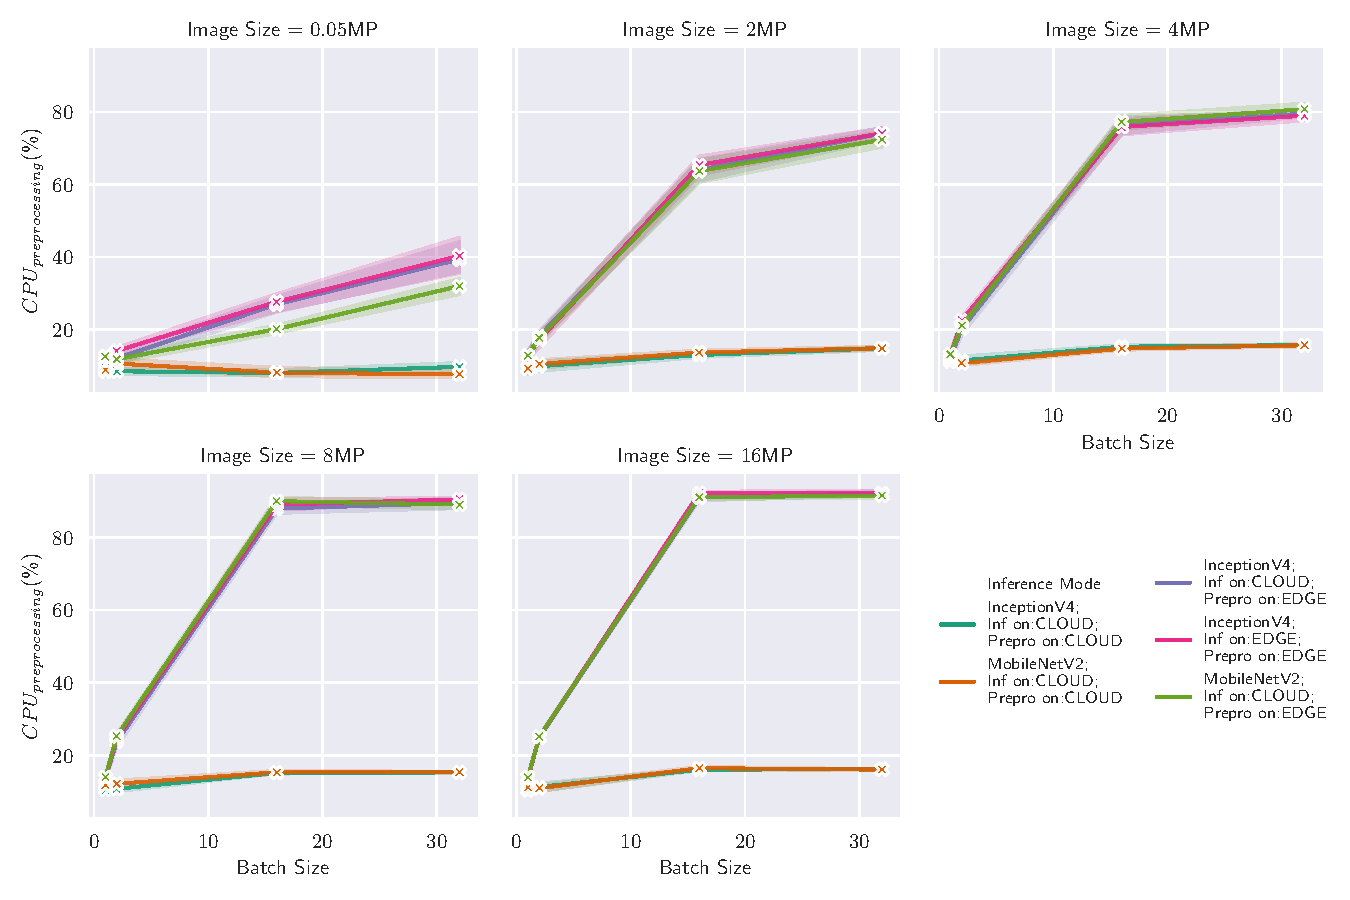
\includegraphics[width=0.95\textwidth]{./Bilder/single_plots/batch_size_plots/Effects_of_Batch_size_Preprocessing_CPU_Usage.pdf}
\caption{Edge vs. Cloud Inference for larger Batch Sizes -  $CPU_{preprocessing}$}
\label{fig:BatchSizePreproCPU}
\end{figure}

\begin{figure}[H]
\centering
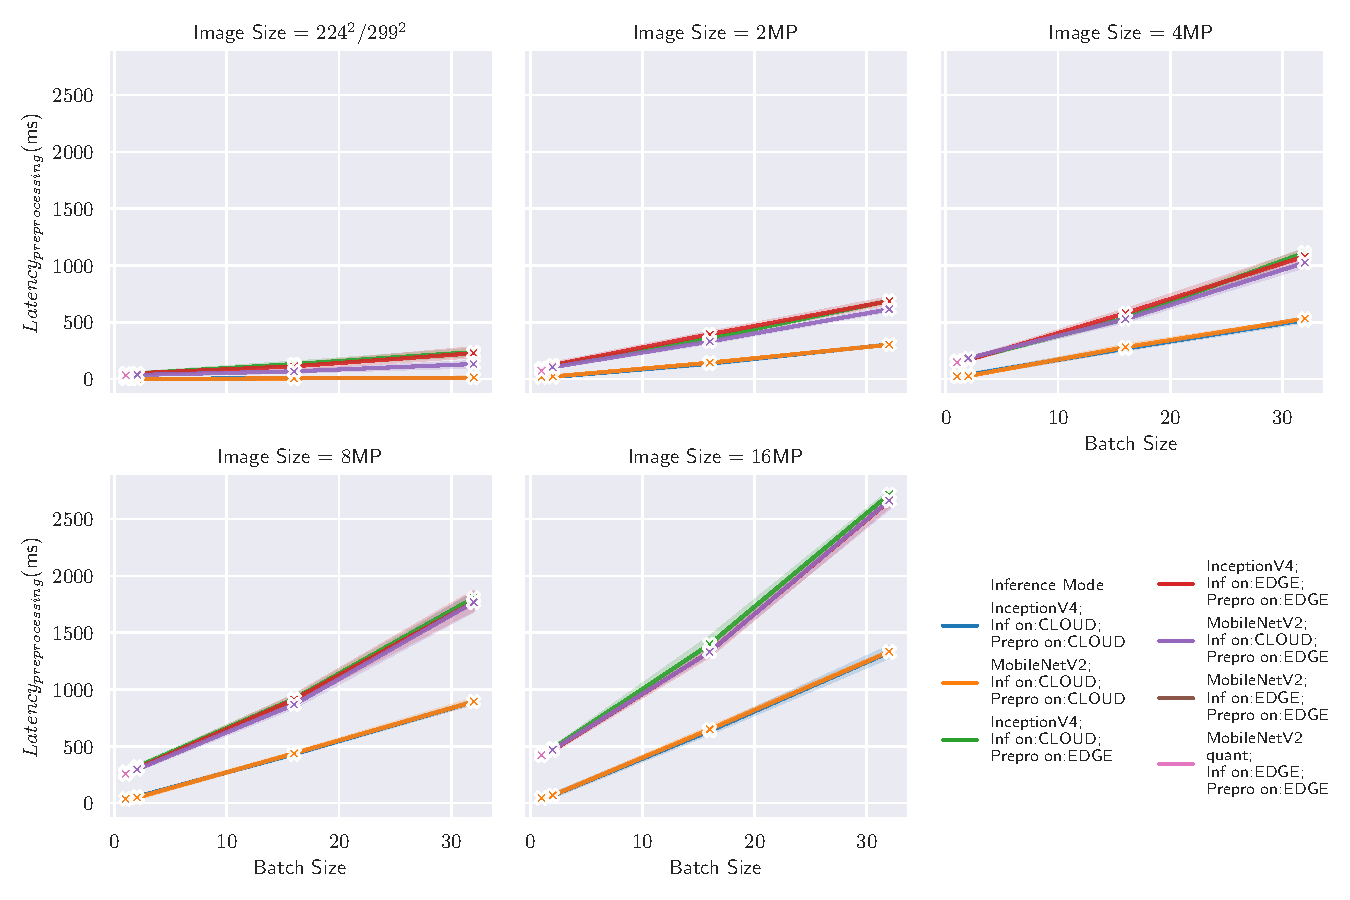
\includegraphics[width=0.95\textwidth]{./Bilder/single_plots/batch_size_plots/Effects_of_Batch_size_Preprocessing_Latencies.pdf}
\caption{Edge vs. Cloud Inference for larger Batch Sizes -  $Latency_{preprocessing}$}
\label{fig:BatchSizePreproLatency}
\end{figure}
\begin{figure}[H]
\centering
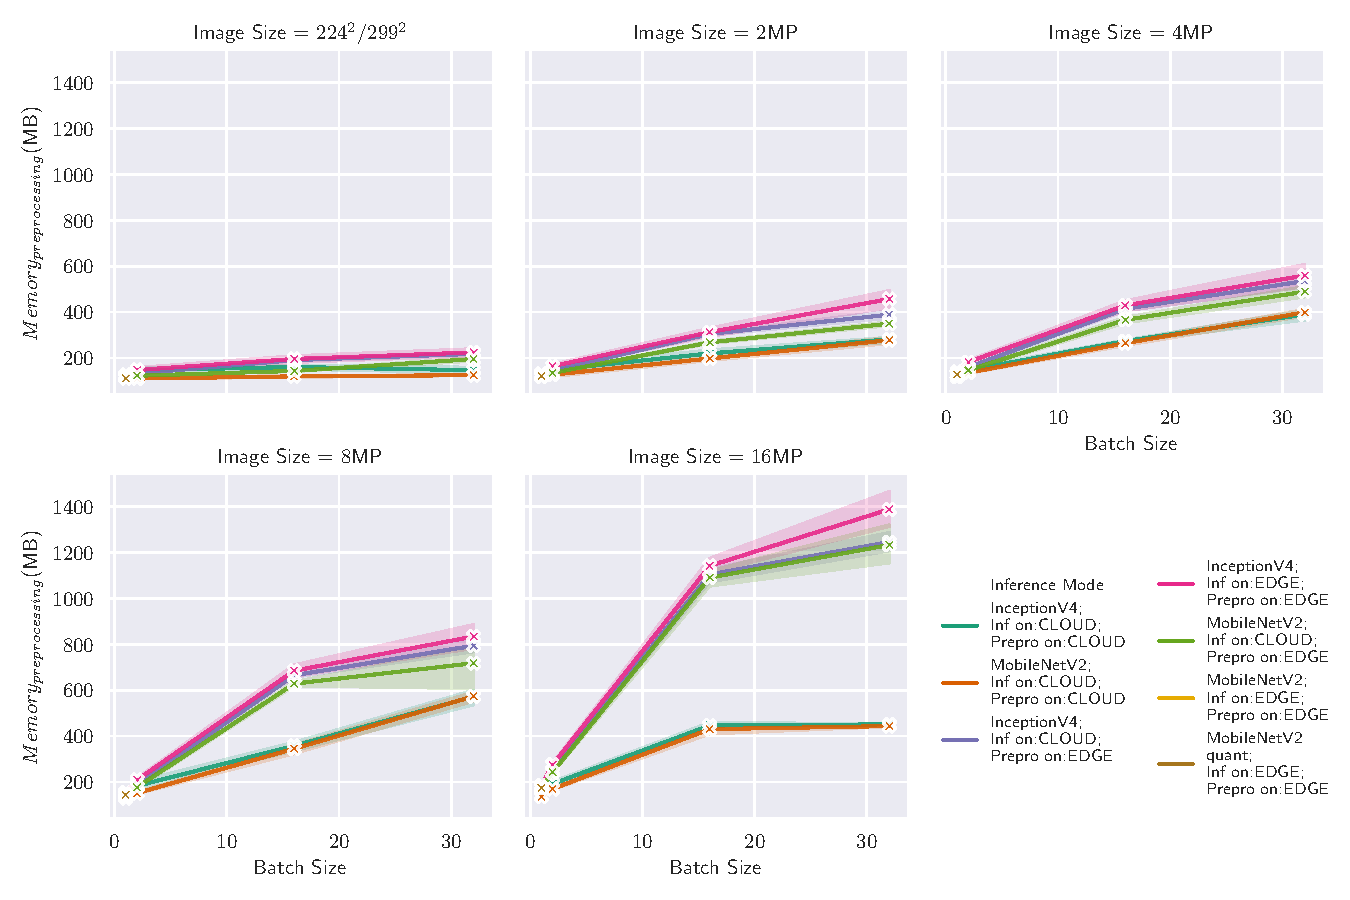
\includegraphics[width=0.95\textwidth]{./Bilder/single_plots/batch_size_plots/Effects_of_Batch_size_Preprocessing_Memory.pdf}
\caption{Edge vs. Cloud Inference for larger Batch Sizes -  $Memory_{preprocessing}$}
\label{fig:BatchSizePreproMemory}
\end{figure}


\subsubsection{Inference}

\begin{figure}[H]
\centering
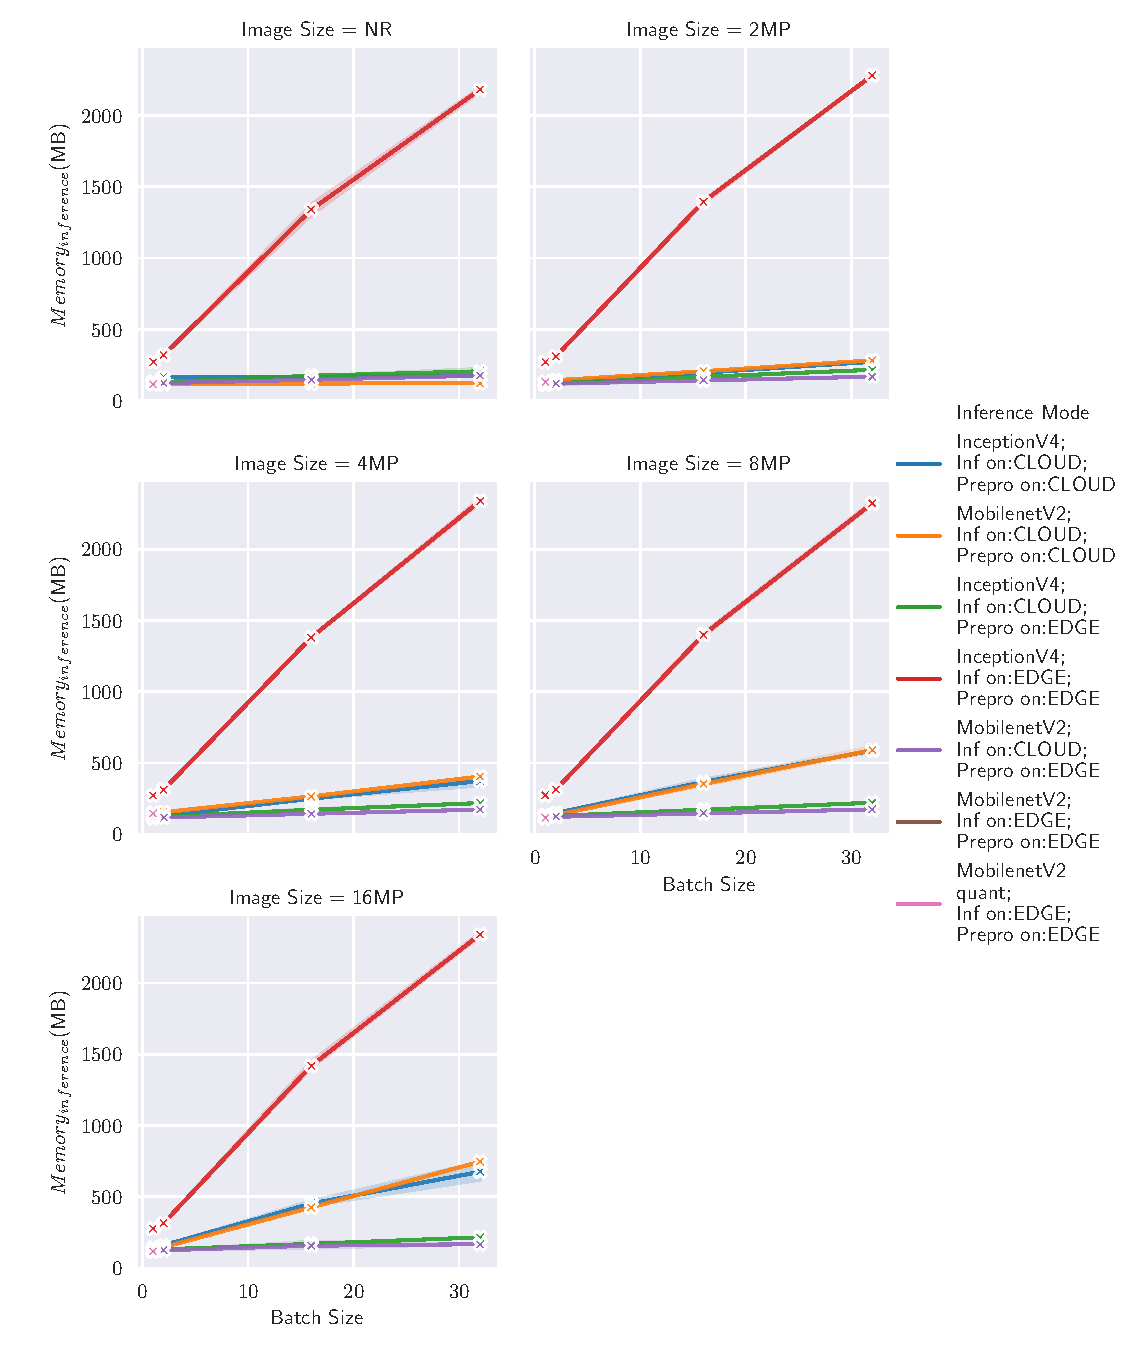
\includegraphics[width=0.95\textwidth]{./Bilder/single_plots/batch_size_plots/Effects_of_Batch_size_Inference_Memory.pdf}
\caption{Edge vs. Cloud Inference for larger Batch Sizes -  $Memory_{inference}$}
\label{fig:BatchSizeInferenceMemory}
\end{figure}
\begin{figure}[H]
\centering
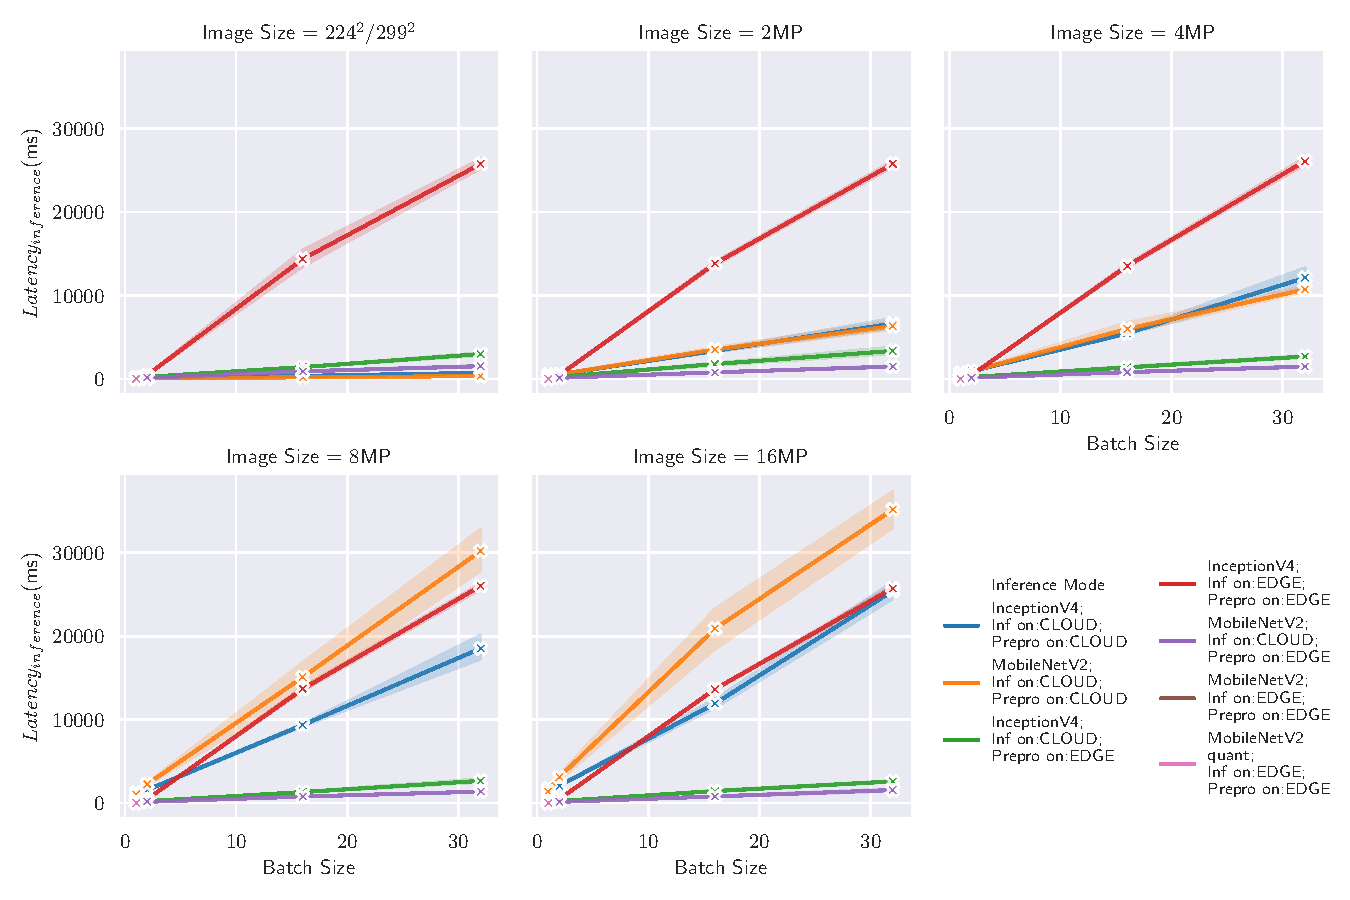
\includegraphics[width=0.95\textwidth]{./Bilder/single_plots/batch_size_plots/Effects_of_Batch_size_Inference_Latencies.pdf}
\caption{Edge vs. Cloud Inference for larger Batch Sizes -  $Latency_{inference}$}
\label{fig:BatchSizeInferenceLatency}
\end{figure}
\begin{figure}[H]
\centering
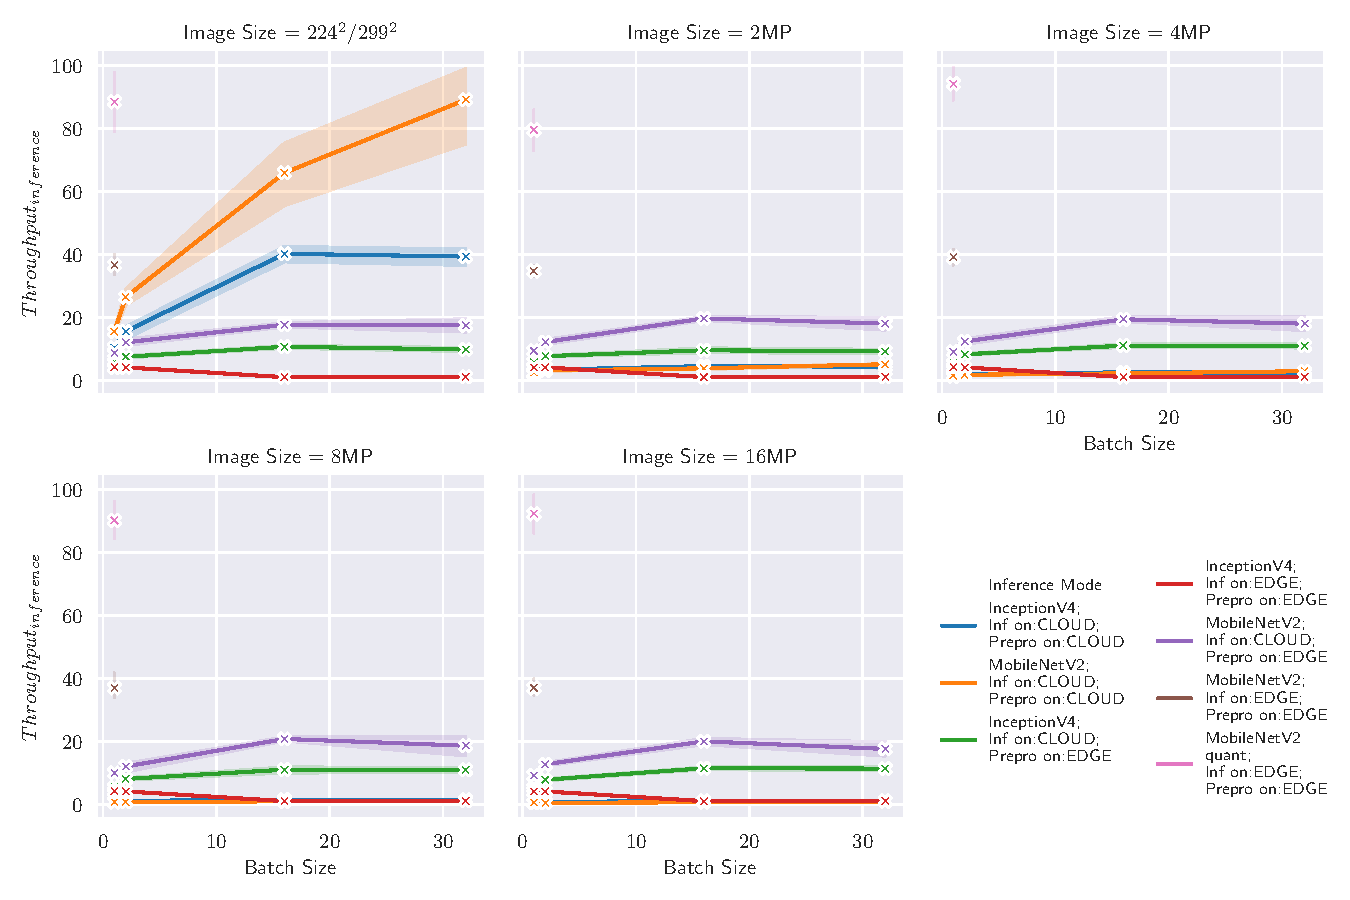
\includegraphics[width=0.95\textwidth]{./Bilder/single_plots/batch_size_plots/Effects_of_Batch_size_Inference_Throughput.pdf}
\caption{Edge vs. Cloud Inference for larger Batch Sizes -  $Throughput_{inference}$}
\label{fig:BatchSizeInferenceThroughput}
\end{figure}





%%%%%%%%%%%%%%%%%%%%%%%%%
%Überleitung

\endinput 
